\documentclass[UTF8,fontset=windows,zihao=-4,openany]{ctexrep}

\usepackage[a4paper,left=2.8cm,right=2.5cm,top=2.6cm,bottom=2.6cm]{geometry}
\usepackage{graphicx}
\usepackage{array}
\usepackage{booktabs}
\usepackage{longtable}
\usepackage{tabularx}
\usepackage{enumitem}
\usepackage{fancyhdr}
\usepackage{titlesec}
\usepackage{xcolor}
\usepackage{hyperref}
\usepackage{listings}
\usepackage{float}
\usepackage{caption}
\usepackage{framed}

\hypersetup{
  colorlinks=true,
  linkcolor=black,
  urlcolor=blue,
  citecolor=black,
  pdfauthor={Agentic Study System 项目组},
  pdftitle={基于大模型的个性化学习资源生成与学习多智能体系统详细设计说明书}
}

\pagestyle{fancy}
\fancyhf{}
\lhead{个性化学习多智能体系统详细设计说明书}
\rhead{\thepage}
\renewcommand{\headrulewidth}{0.4pt}
\setlength{\headheight}{15pt}
\emergencystretch=2em

\setlist[itemize]{leftmargin=2em,itemsep=0.2em,topsep=0.2em}
\setlist[enumerate]{leftmargin=2em,itemsep=0.2em,topsep=0.2em}
\renewcommand{\arraystretch}{1.25}
\setlength{\parindent}{2em}
\setlength{\parskip}{0.2em}

\titleformat{\chapter}{\centering\heiti\zihao{3}}{第\chinese{chapter}章}{1em}{}
\titleformat{\section}{\heiti\zihao{4}}{\thesection}{0.8em}{}
\titleformat{\subsection}{\heiti\zihao{-4}}{\thesubsection}{0.8em}{}

\lstdefinestyle{codestyle}{
  basicstyle=\ttfamily\small,
  breaklines=true,
  columns=fullflexible,
  frame=single,
  numbers=none,
  backgroundcolor=\color{gray!6},
  rulecolor=\color{gray!40}
}
\lstset{style=codestyle}

\newcolumntype{Y}{>{\raggedright\arraybackslash}X}

\begin{document}

\begin{titlepage}
  \centering
  \vspace*{2.0cm}
  {\zihao{1}\heiti 基于大模型的个性化学习资源生成\\[0.4em]与学习多智能体系统\par}
  \vspace{1.5cm}
  {\zihao{2}\heiti 详细设计说明书\par}
  \vspace{3.0cm}
  \begin{tabular}{rl}
    项目名称： & Agentic Study System\\
    文档类型： & 详细设计说明书\\
    编写日期： & 2026 年 6 月\\
    适用对象： & 设计人员、开发人员、测试人员、部署维护人员\\
  \end{tabular}
\end{titlepage}

\pagenumbering{Roman}
\tableofcontents
\clearpage
\pagenumbering{arabic}

\chapter{引言}

\section{编写目的}

本说明书围绕 Agentic Study System 的系统结构、模块边界、接口约定、运行流程、文件数据结构、异常处理、安全控制和优化方向进行详细设计说明，为系统开发、测试、部署和维护提供依据。

与传统课程资料管理系统相比，本项目不是简单地保存课件和笔记，而是围绕“课程资料接入、知识生成、测评反馈、学习画像、个性化路径、检索问答”形成闭环。因此，系统设计重点放在多智能体协作、模型路由、文件化状态管理、RAG 回退机制和中文内容质量控制上。

\section{项目背景}

高校课程学习场景中，学生通常面临三个典型问题：课程资料数量多、抽象概念理解门槛高、复习和反馈缺乏个性化。传统学习工具通常只能提供资料存储、题库练习或单轮问答，难以持续跟踪学生画像、知识短板和学习路径。

Agentic Study System 面向上述场景构建本地化学习工作台。用户导入课程 PDF 后，系统通过 PDF 解析、OCR、分层讲义生成、知识图解、拓展材料、智能测评、诊断反馈、学习画像和 RAG 问答等模块，为同一门课程持续生成可阅读、可练习、可追踪、可问答的学习资源。系统采用 FastAPI 提供本地 Web 服务，前端使用原生 HTML/CSS/JavaScript，后端使用 Python 智能体模块完成业务编排，并通过统一的 LLMRouter 对接 OpenAI、Anthropic、vLLM、Ollama 和 LightRAG 等服务。

从工程实现角度看，本项目并不是单一的“聊天问答”应用，而是由 Web 服务、文档解析、OCR、知识检索、内容生成、结构化校验和文件化存储共同组成的学习资源生产系统。FastAPI 的异步接口模型适合处理上传、状态查询和外部 API 等 I/O 密集型操作；PyMuPDF 提供 PDF 文本抽取与页面渲染能力；Tesseract OCR 用于补足扫描版或图片型 PDF 的可读文本；Mermaid 使知识图解可以直接以 Markdown 代码块形式保存和渲染；LightRAG 则为课程资料问答提供可选的图结构增强检索思路。上述技术共同支撑了“资料进入系统后持续转化为学习产物”的核心目标。

\section{预期读者与阅读建议}

\begin{longtable}{p{0.22\textwidth}p{0.68\textwidth}}
\toprule
预期读者 & 阅读重点\\
\midrule
系统设计人员 & 总体架构、设计原则、模块边界、多智能体协作方式、数据流与控制流。\\
开发人员 & 核心模块职责、接口设计、文件数据结构、模型路由、异常与安全处理。\\
测试人员 & 功能流程、接口输入输出、运行控制、测试用例设计和质量约束。\\
部署维护人员 & 环境依赖、运行方式、LightRAG/OCR/模型服务配置、出错处理和日志位置。\\
项目管理与评审人员 & 项目背景、功能范围、系统优势和优化方向。\\
\bottomrule
\end{longtable}

\section{参考资料}

参考资料如下：
\begin{enumerate}
  \item 项目 README：\texttt{README.md}。
  \item 项目使用与测试说明：\texttt{docs/USAGE\_AND\_TESTING\_ZH.md}。
  \item 关键源码文件：\texttt{main.py}、\texttt{webapp/server.py}、\texttt{core/*.py}、\texttt{agents/*.py}、\texttt{config.yaml}。
  \item FastAPI 官方文档：异步接口、静态文件服务与测试支持，\url{https://fastapi.tiangolo.com/async/}，\url{https://fastapi.tiangolo.com/tutorial/static-files/}。
  \item Uvicorn 官方文档：ASGI 服务运行方式，\url{https://www.uvicorn.org/}。
  \item PyMuPDF 官方文档：页面文本抽取与页面图像渲染接口，\url{https://pymupdf.readthedocs.io/en/latest/page.html}。
  \item Tesseract OCR 官方文档：训练数据和语言包说明，\url{https://tesseract-ocr.github.io/tessdoc/Data-Files.html}。
  \item Mermaid 官方文档：Markdown 图表语法与渲染能力，\url{https://mermaid.js.org/intro/}。
  \item LightRAG 论文资料：\textit{LightRAG: Simple and Fast Retrieval-Augmented Generation}，\url{https://arxiv.org/abs/2410.05779}。
  \item OpenAI API 官方参考：Chat/模型调用接口说明，\url{https://developers.openai.com/api/reference/resources/chat}。
\end{enumerate}

\chapter{总体设计}

\section{需求规定}

\subsection{对功能的规定}

系统应支持以下核心功能：

\begin{enumerate}
  \item 课程管理。支持课程新建、选择、重命名和删除；每门课程拥有独立章节、诊断记录、学习画像、行为日志和个性化学习路径。
  \item PDF 资料接入。支持在 Web 页面上传课程 PDF，系统自动创建新章节或写入指定章节的 \texttt{input} 目录。
  \item 课程资料解析。支持从 PDF 中提取文本并渲染页面图片；当页面文本过少时调用 Tesseract OCR 进行中文和英文识别。
  \item 分层讲义生成。围绕同一章节生成 \texttt{Beginner.md}、\texttt{Intermediate.md}、\texttt{Advanced.md} 三类中文讲义。
  \item 知识图解生成。根据三层讲义提取主要概念，生成包含 Mermaid 结构图的 \texttt{Diagrams.md}。
  \item 拓展材料生成。基于讲义与图解生成 \texttt{Extension.md}，用于补充阅读、实践案例和复习建议。
  \item 智能测评。生成结构化题库 \texttt{Quiz.json} 和可读题面 \texttt{Quiz.md}，支持客观题即时检查和开放题深度反馈。
  \item 诊断反馈。学生提交 \texttt{Answers.md} 或综合论述后，系统生成 \texttt{Feedback.md}，并把关键发现追加到课程级 \texttt{Diagnostic.md}。
  \item 学习画像。支持用户手动填写画像，或由 Profile Agent 根据访谈记录、诊断记录和章节状态更新 \texttt{Profile.json}/\texttt{Profile.md}。
  \item 个性化学习路径。基于学习画像、诊断记录和章节状态生成 \texttt{LearningPath.md}。
  \item 课程资料问答。支持接入 LightRAG Server 进行增强检索；当 LightRAG 未配置或调用失败时，自动回退到本地 Markdown/PDF 分块检索。
  \item 学习行为记录与推荐。系统将主要学习事件写入 \texttt{BehaviorLog.jsonl}，并通过规则生成下一步推荐。
\end{enumerate}

\subsection{对性能的规定}

系统定位为本地单用户或小规模教学辅助系统，性能要求以稳定可用和长任务可观察为主：
\begin{itemize}
  \item Web 页面状态查询、文件读取、课程列表刷新等轻量接口应在秒级内返回；此类接口不应等待模型生成、OCR 或大文件解析完成。
  \item PDF 解析、OCR、讲义生成、题库生成等长任务允许耗时较长，但应通过异步线程、流式进度或明确的前端等待状态避免阻塞 Web 服务事件循环。
  \item RAG 问答在 LightRAG 可用时优先使用外部增强检索；失败时应快速回退到本地检索，并把回退原因返回给前端，保证问答功能不完全失效。
  \item 文档解析与图像渲染应避免一次性保留过多大对象；多页 PDF 应按页处理、按章节保存中间结果，降低本地运行环境的内存压力。
  \item 文件写入应采用 UTF-8 编码，避免中文讲义、题库、诊断和画像出现乱码。
  \item 模型调用失败时应返回可理解的错误信息，包括缺失 API Key、模型不存在、Ollama 未启动、vLLM 隧道未打开等情况。
\end{itemize}

\subsection{对兼容性的规定}

系统主要面向 Windows 本地开发和教学运行环境，同时具备跨平台 Python 项目的基础可迁移性。
\begin{itemize}
  \item 后端应支持 Python 3.11 或更高版本。
  \item Web 前端应支持 Chrome、Edge、Firefox 等现代浏览器。
  \item PDF 解析依赖 PyMuPDF；OCR 能力依赖系统级 Tesseract 与语言包。
  \item LLM 服务可通过 OpenAI、Anthropic、自部署 vLLM 或 Ollama 接入，具体模型由 \texttt{config.yaml} 和 \texttt{.env} 决定。
  \item LightRAG 为可选增强能力，不应成为主系统启动的硬依赖。
\end{itemize}

\subsection{界面要求}

系统界面应围绕学习工作台而非营销页面设计，首页即展示可操作的课程驾驶舱。主要界面包括：
\begin{itemize}
  \item 课程侧栏：展示当前课程、课程操作按钮、资料接入区和章节流程列表。
  \item 资源中心：预览分层讲义、知识图解、拓展材料、测评反馈等 Markdown 内容，并渲染 Mermaid 图。
  \item 智能测评页签：展示题库、客观题检查、开放题作答、深度反馈入口和综合论述保存区域。
  \item 知识问答页签：提供问题输入框、RAG 模式选择、索引全部课程资料按钮和答案展示区。
  \item 学习画像页签：提供画像字段表单、访谈记录输入、AI 提取画像、生成学习计划和查看学习计划功能。
  \item 学习诊断入口：展示课程级 \texttt{Diagnostic.md} 中持续积累的学习反馈。
\end{itemize}

\section{开发与运行环境}

\subsection{开发环境}

\begin{longtable}{p{0.25\textwidth}p{0.62\textwidth}}
\toprule
类别 & 内容\\
\midrule
主要语言 & Python、JavaScript、HTML、CSS、Markdown、YAML\\
后端框架 & FastAPI、Uvicorn\\
前端技术 & 原生 HTML/CSS/JavaScript，内置 marked 与 Mermaid 静态资源\\
PDF 处理 & PyMuPDF\\
OCR & pytesseract 与 Tesseract OCR，可配置 \texttt{chi\_sim+eng}\\
模型接入 & OpenAI SDK、Anthropic SDK、Ollama、OpenAI-compatible vLLM\\
RAG 增强 & 内嵌 LightRAG 源码，可启动独立 LightRAG Server\\
配置管理 & \texttt{config.yaml} 与 \texttt{.env}\\
数据保存 & 文件系统目录、Markdown、JSON、JSONL、PDF、PNG\\
\bottomrule
\end{longtable}

\subsection{运行环境}

主系统运行入口为：

\begin{lstlisting}[language=bash]
python main.py serve --port 8000
\end{lstlisting}

浏览器访问地址为：

\begin{lstlisting}
http://127.0.0.1:8000
\end{lstlisting}

如需 LightRAG 增强检索，可单独启动 LightRAG Server，并在 \texttt{.env} 中配置 \texttt{LIGHTRAG\_BASE\_URL}。如需 OCR 扫描版 PDF，应在系统 PATH 中安装 Tesseract OCR 和中文语言包。

\section{关键技术选型依据}

项目技术选型以“低部署门槛、文件产物可检查、生成流程可降级”为主要约束。各关键技术的职责边界如下表所示。

\begin{longtable}{p{0.22\textwidth}p{0.30\textwidth}p{0.36\textwidth}}
\toprule
技术组件 & 选型依据 & 在本系统中的设计边界\\
\midrule
FastAPI + Uvicorn & FastAPI 支持异步路径操作、自动接口文档和静态资源挂载；Uvicorn 作为 ASGI 服务器适合本地快速启动。 & 只承担 HTTP 接口、静态文件服务、上传处理、状态聚合和长任务调度，不把智能体逻辑写入路由函数。\\
PyMuPDF & 官方接口支持页面文本抽取和页面图像渲染，便于同时处理文本型 PDF 与 OCR 所需图片。 & 负责从 \texttt{input/*.pdf} 生成章节文本和页面图片，不负责语义总结，避免解析层与生成层耦合。\\
Tesseract OCR & 通过语言数据文件支持多语言 OCR，可在本地完成扫描版资料识别。 & 作为文本层不足时的补救机制；OCR 不可用时不阻断系统启动，而是给出安装提示。\\
Markdown + Mermaid & Markdown 便于人工阅读、版本管理和前端渲染；Mermaid 可用文本描述流程图、结构图和知识图。 & 学习资料、图解、反馈和路径以文本文件保存，前端负责渲染；生成器需保证 Mermaid 代码块可解析。\\
LightRAG & LightRAG 提供轻量级检索增强生成思路，适合扩展课程资料问答的关系检索能力。 & 定位为可选增强服务；不可用时回退到本地 Markdown/PDF 分块检索。\\
LLMRouter & 统一屏蔽 OpenAI、Anthropic、vLLM、Ollama 等不同模型服务的调用差异。 & 智能体只声明逻辑路由，不直接持有密钥、模型地址和供应商细节。\\
\bottomrule
\end{longtable}

\section{设计原则}

\begin{enumerate}
  \item 模块化原则。课程管理、资料解析、资源生成、测评反馈、画像路径、RAG 问答和模型路由均采用独立模块，降低耦合度。
  \item 文件可追溯原则。系统生成的所有核心学习产物均以 Markdown、JSON 或 JSONL 形式保存在课程目录中，便于查看、复制、测试和复现。
  \item 模型路由统一原则。所有大模型调用均通过 \texttt{core/llm\_router.py}，避免各智能体直接硬编码模型和服务地址。
  \item 可降级原则。LightRAG、OCR、外部大模型均可能不可用，系统应提供本地检索、文本 PDF 解析、清晰错误提示等降级路径。
  \item 中文内容质量原则。系统输出以简体中文为主，关键生成任务使用校验器避免乱码、韩文残留、缺少 Mermaid 图、先讲抽象定义后给例子等问题。
  \item 安全与隐私原则。本地密钥保存在 \texttt{.env} 且被 Git 忽略；对保存接口进行文件白名单限制；对用户文件名进行路径穿越校验。
\end{enumerate}

\section{设计思想}

系统整体采用“薄编排层 + 多智能体业务层 + 文件化共享状态 + 可选知识库增强”的设计思想。FastAPI 只负责接口、上传、文件读取、长任务调度和状态聚合；具体的知识生成、测评和画像更新由各智能体承担；智能体之间不直接共享大段上下文，而是通过文件路径和简短状态摘要衔接；课程目录既是用户可见的学习资料库，也是系统内部的状态库。

该设计适合课程学习场景。一方面，Markdown 和 JSON 便于学生、教师或测试人员直接检查内容；另一方面，多智能体可围绕不同学习任务使用不同提示词、模型路由和校验规则，避免把所有功能塞入单个复杂提示词中。

具体而言，系统在实现上强调四个层面的分离：
\begin{enumerate}
  \item 接口层与业务层分离。Web 路由只接收请求、校验参数并调度业务对象，学习资源生成逻辑集中在智能体和核心模块中。
  \item 原始资料与生成产物分离。PDF 原件、解析文本、页面图片、讲义、题库、反馈和画像分别保存，便于追踪错误来自解析阶段还是生成阶段。
  \item 增强能力与基础能力分离。LightRAG、OCR 和外部大模型均可提升效果，但系统必须在缺失其中一项时给出可解释的降级行为。
  \item 自动生成与人工检查分离。系统提供结构化校验和安全提示，但课程内容的事实准确性、题目难度和最终发布结果仍保留人工确认入口。
\end{enumerate}

\begin{figure}[H]
  \centering
  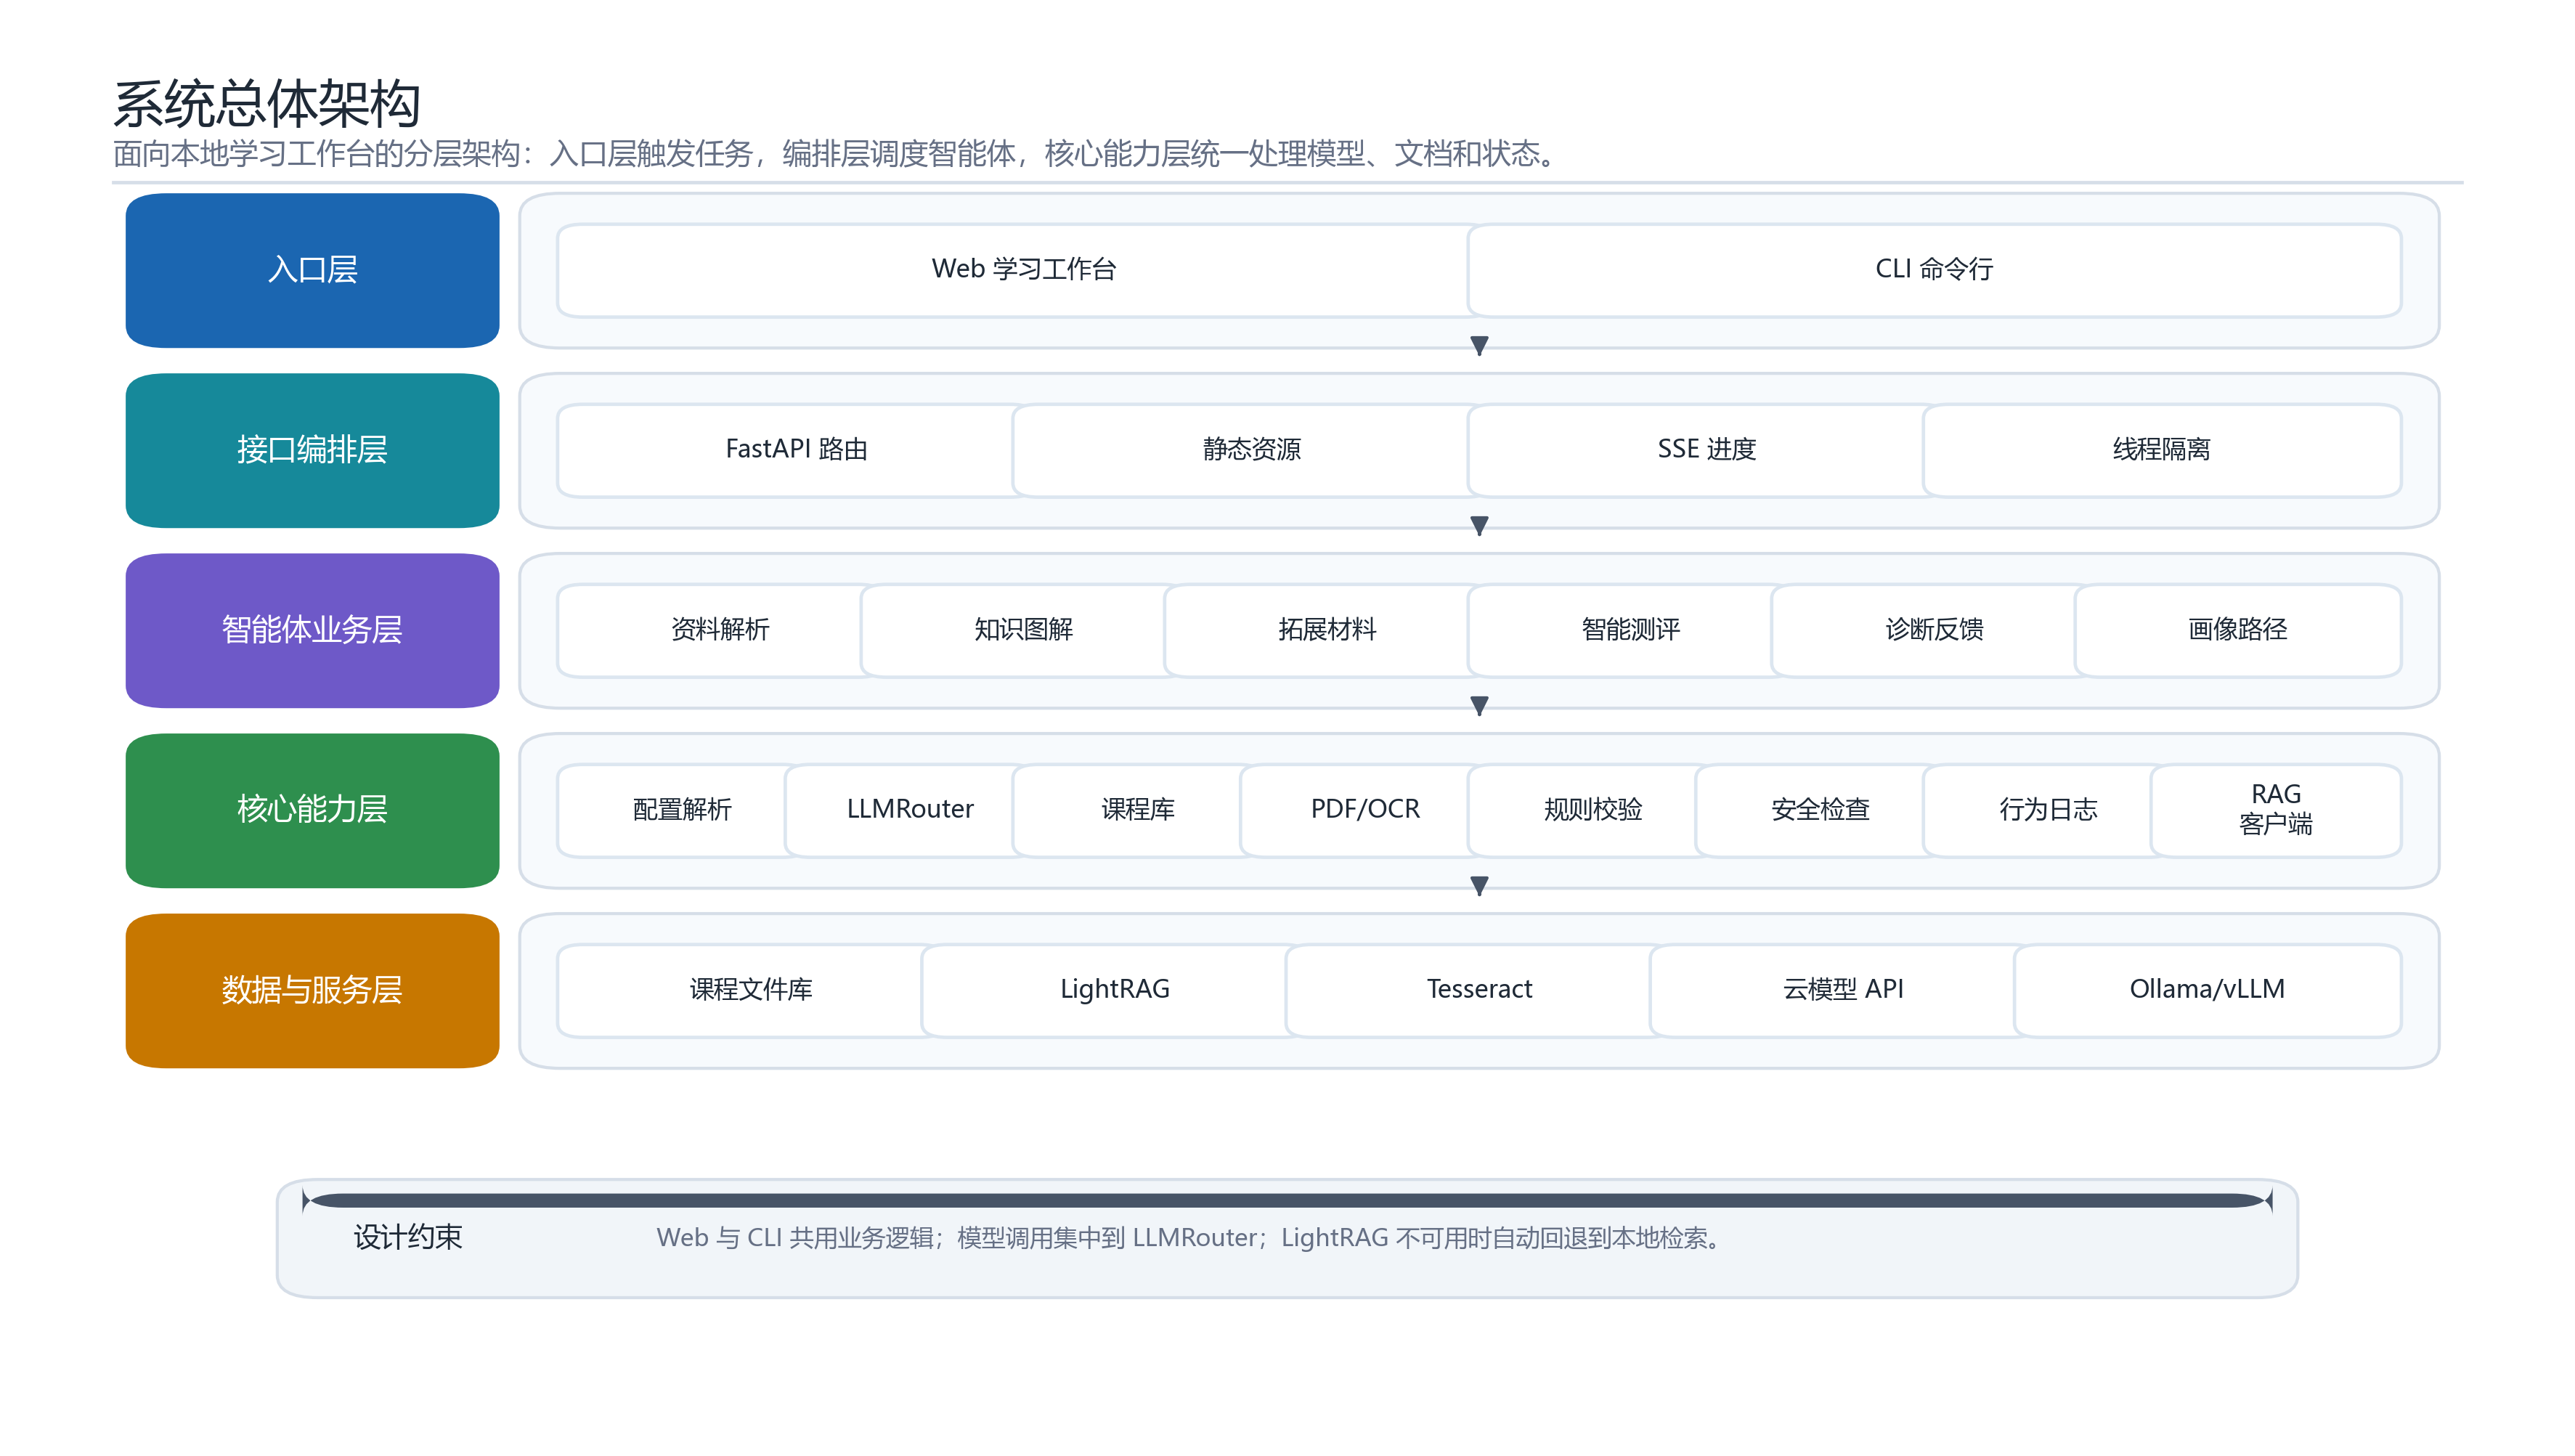
\includegraphics[width=0.98\textwidth]{fig_system_architecture.png}
  \caption{系统总体架构图}
\end{figure}

\chapter{流程设计}

\section{核心业务流程}

系统核心流程围绕一门课程的一个章节展开，形成“输入资料、生成资源、完成测评、获得反馈、更新画像、规划路径”的闭环。

\begin{figure}[H]
  \centering
  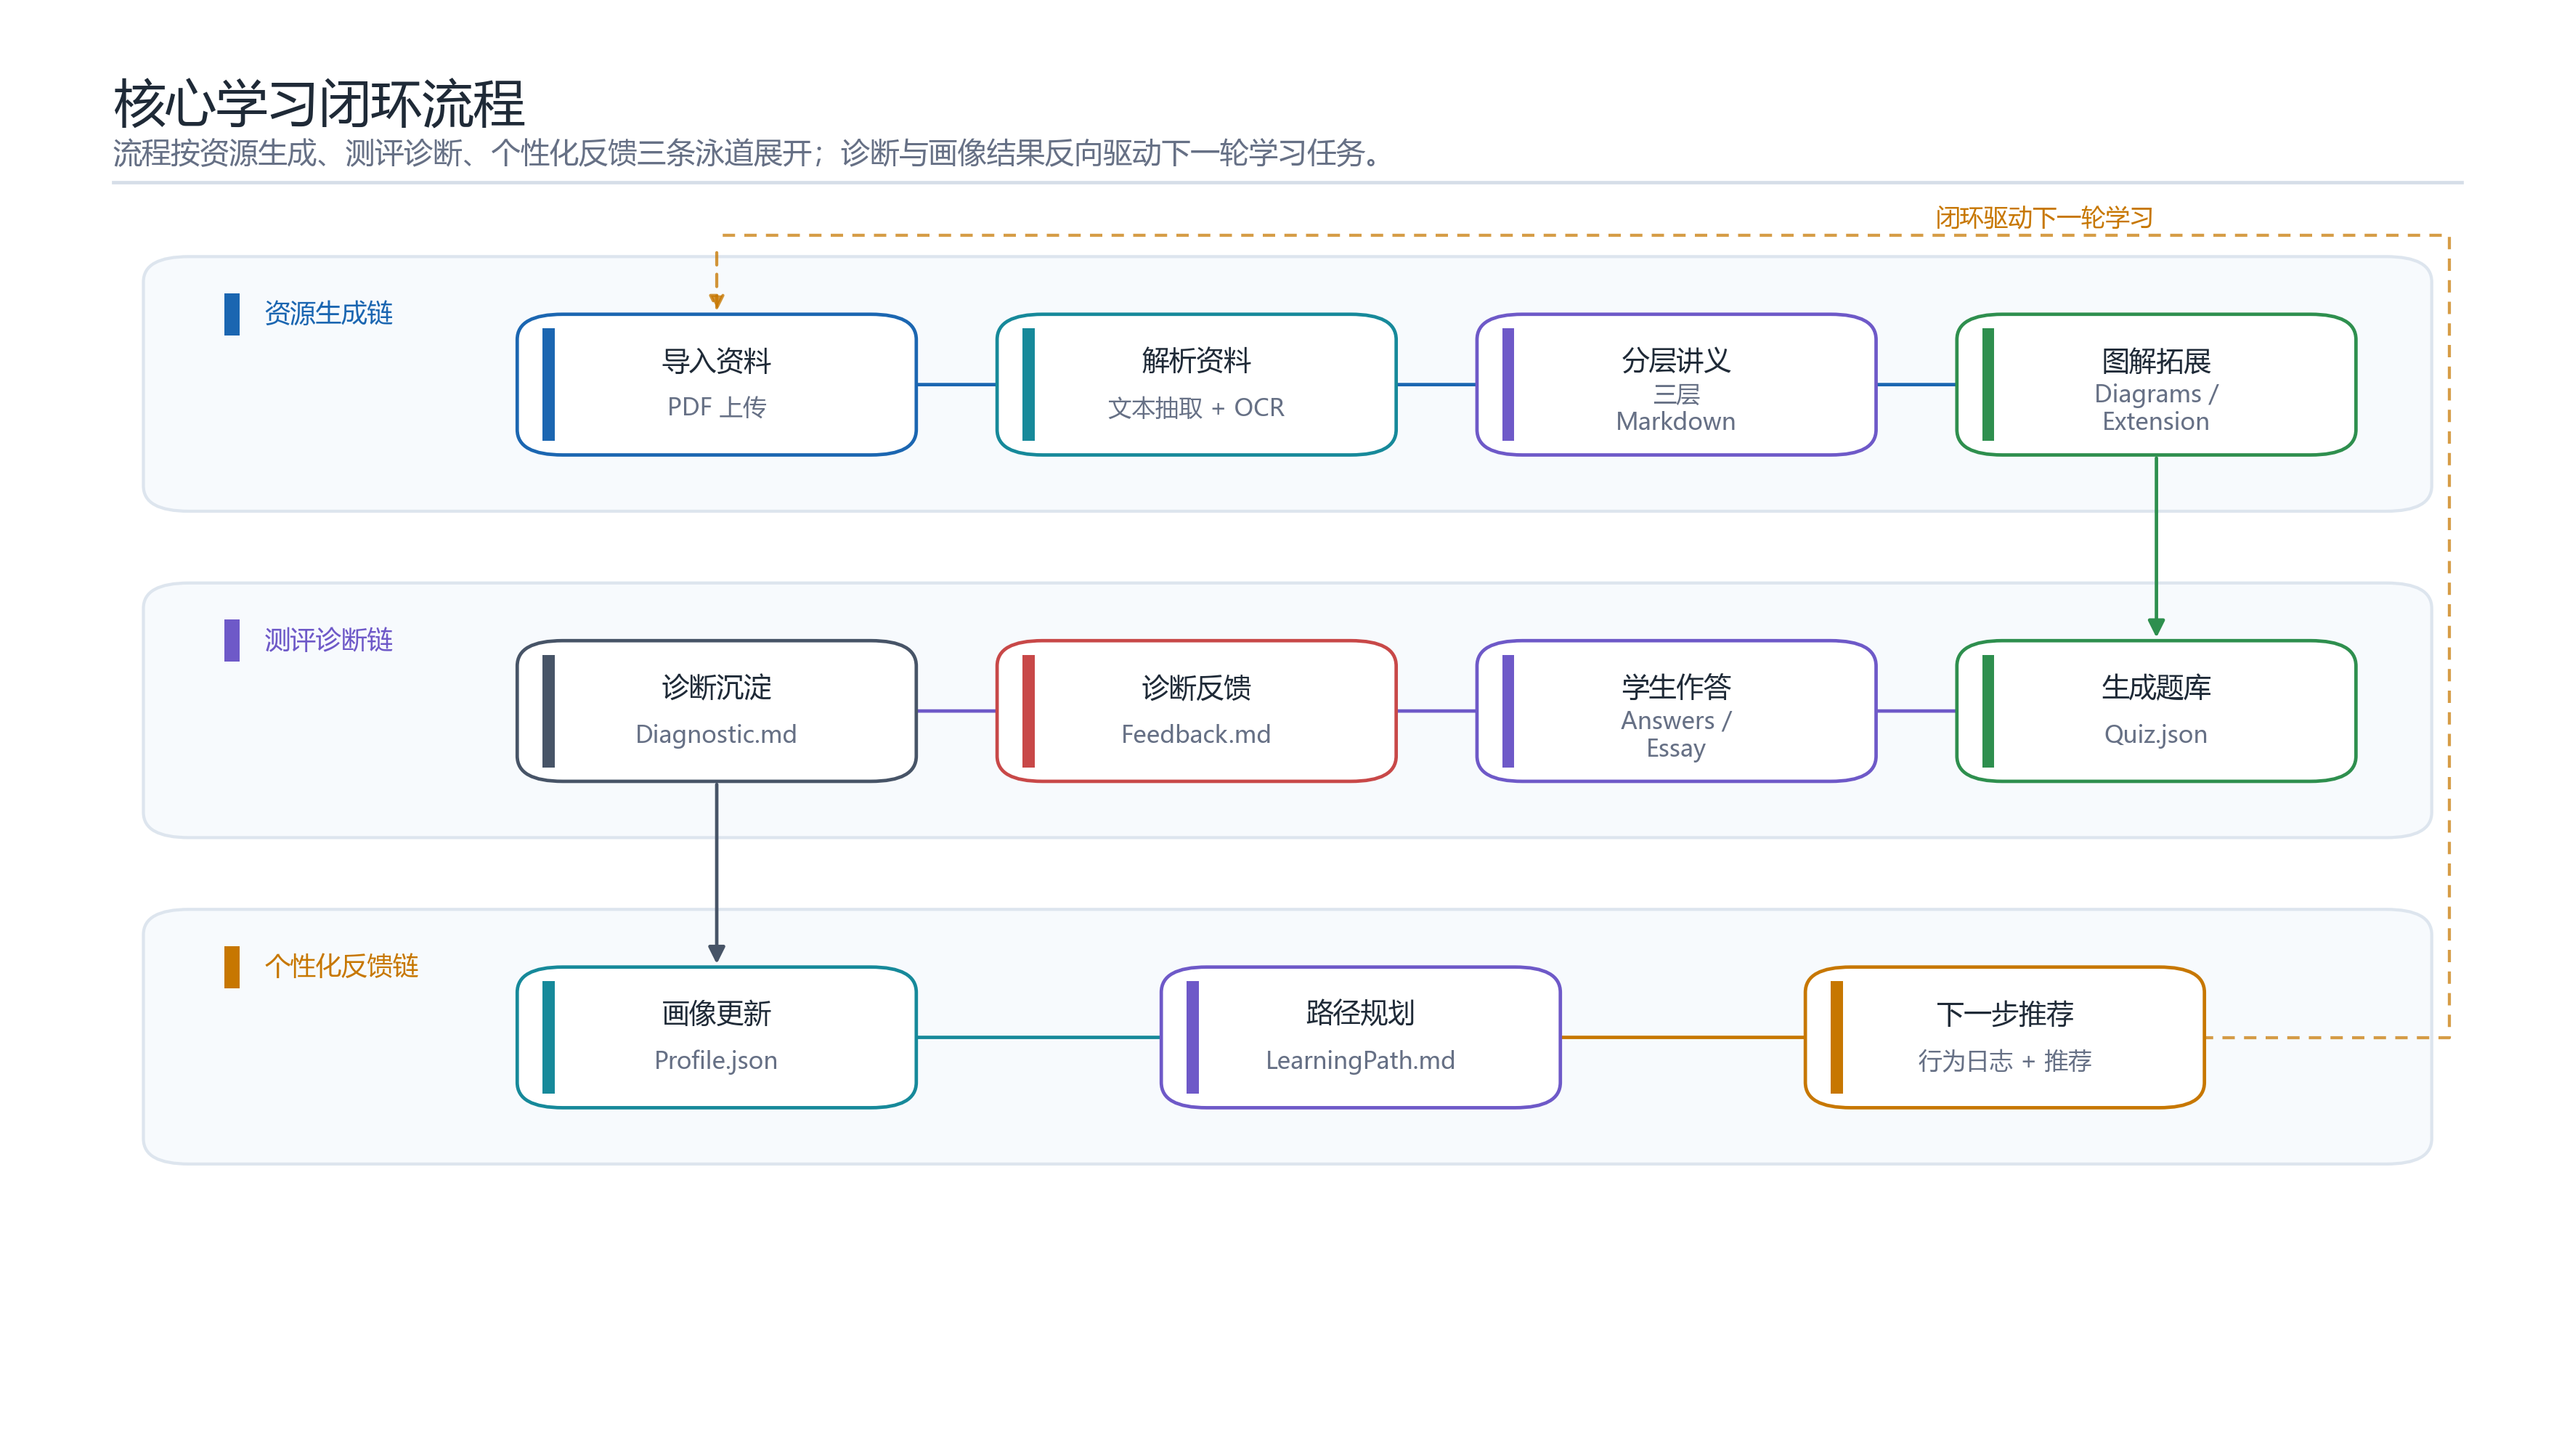
\includegraphics[width=0.98\textwidth]{fig_learning_workflow.png}
  \caption{核心学习业务流程图}
\end{figure}

\subsection{课程创建与资料导入流程}

\begin{enumerate}
  \item 用户在 Web 页面点击“新建课程”，输入课程名称。
  \item 后端调用 \texttt{SubjectStore.create\_subject} 生成课程 slug 和 \texttt{subject.json}。
  \item 用户上传 PDF，前端通过 \texttt{/api/upload} 提交文件。
  \item 后端根据上传目标创建 \texttt{Week\_NN/input} 目录，将 PDF 保存到章节输入目录。
  \item 刷新 \texttt{/api/state} 后，页面显示新章节和 PDF 数量。
\end{enumerate}

\subsection{资料解析与分层讲义生成流程}

\begin{enumerate}
  \item 用户点击章节的生成讲义按钮，前端调用 \texttt{/api/ingest} 或 \texttt{/api/ingest/stream}。
  \item \texttt{IngestionAgent} 读取 \texttt{config.yaml} 中的 OCR 和模型参数。
  \item \texttt{parse\_week\_inputs} 遍历 \texttt{input/*.pdf}，用 PyMuPDF 提取每页文本并渲染页面图片到 \texttt{assets}。
  \item 若页面内嵌文本少于阈值，系统调用 Tesseract OCR 识别页面图片。
  \item 智能体分别按基础层、应用层、提升层提示词生成三份讲义。
  \item 校验器检查中文内容、Mermaid 图块和“先例后理”结构，必要时触发有限次重试。
  \item 输出 \texttt{Beginner.md}、\texttt{Intermediate.md}、\texttt{Advanced.md}。
\end{enumerate}

\subsection{知识图解与拓展材料流程}

当章节已有讲义后，用户可生成知识图解和拓展材料。
\begin{itemize}
  \item 知识图解由 \texttt{WebExplorer} 从讲义标题和内容中提取概念，生成 Mermaid 知识结构图和图解说明，写入 \texttt{Diagrams.md}。
  \item 拓展材料由 \texttt{ExtensionAgent} 综合三层讲义和图解内容，生成拓展阅读、案例、实践建议等内容，写入 \texttt{Extension.md}。
\end{itemize}

\subsection{智能测评与诊断反馈流程}

\begin{enumerate}
  \item 用户点击测评入口，系统读取本章节的三层讲义。
  \item \texttt{QuizAgent} 根据配置数量生成结构化题库，输出 \texttt{Quiz.json}、\texttt{Quiz.md} 和空白 \texttt{Answers.md} 模板。
  \item 前端读取 \texttt{Quiz.json}，对单选题和填空题进行客户端即时检查，对简答题和综合题提供参考答案或开放作答区。
  \item 用户保存答案或综合论述，后端仅允许写入 \texttt{Answers.md} 和 \texttt{Essay.md} 两类文件。
  \item 用户提交深度反馈后，\texttt{GraderAgent} 读取题目和答案，生成 \texttt{Feedback.md}。
  \item 反馈中的知识缺口和薄弱项被抽取后追加到课程级 \texttt{Diagnostic.md}。
\end{enumerate}

\subsection{学习画像与路径规划流程}

画像和路径规划是系统个性化能力的核心。
\begin{enumerate}
  \item 用户可直接在页面表单填写专业背景、学习目标、知识基础、认知风格、短板、兴趣和资源偏好。
  \item 用户也可输入访谈记录，由 \texttt{ProfileAgent} 结合当前画像、诊断文本和章节状态生成新的画像 JSON。
  \item \texttt{save\_profile} 将画像规范化后保存为 \texttt{Profile.json}，并渲染为 \texttt{Profile.md}。
  \item \texttt{PathPlannerAgent} 基于 \texttt{Profile.md}、\texttt{Diagnostic.md} 和章节状态生成 \texttt{LearningPath.md}。
  \item \texttt{recommendations.py} 根据课程状态、画像缺失和行为事件生成可立即执行的下一步推荐。
\end{enumerate}

\subsection{RAG 问答流程}

\begin{figure}[H]
  \centering
  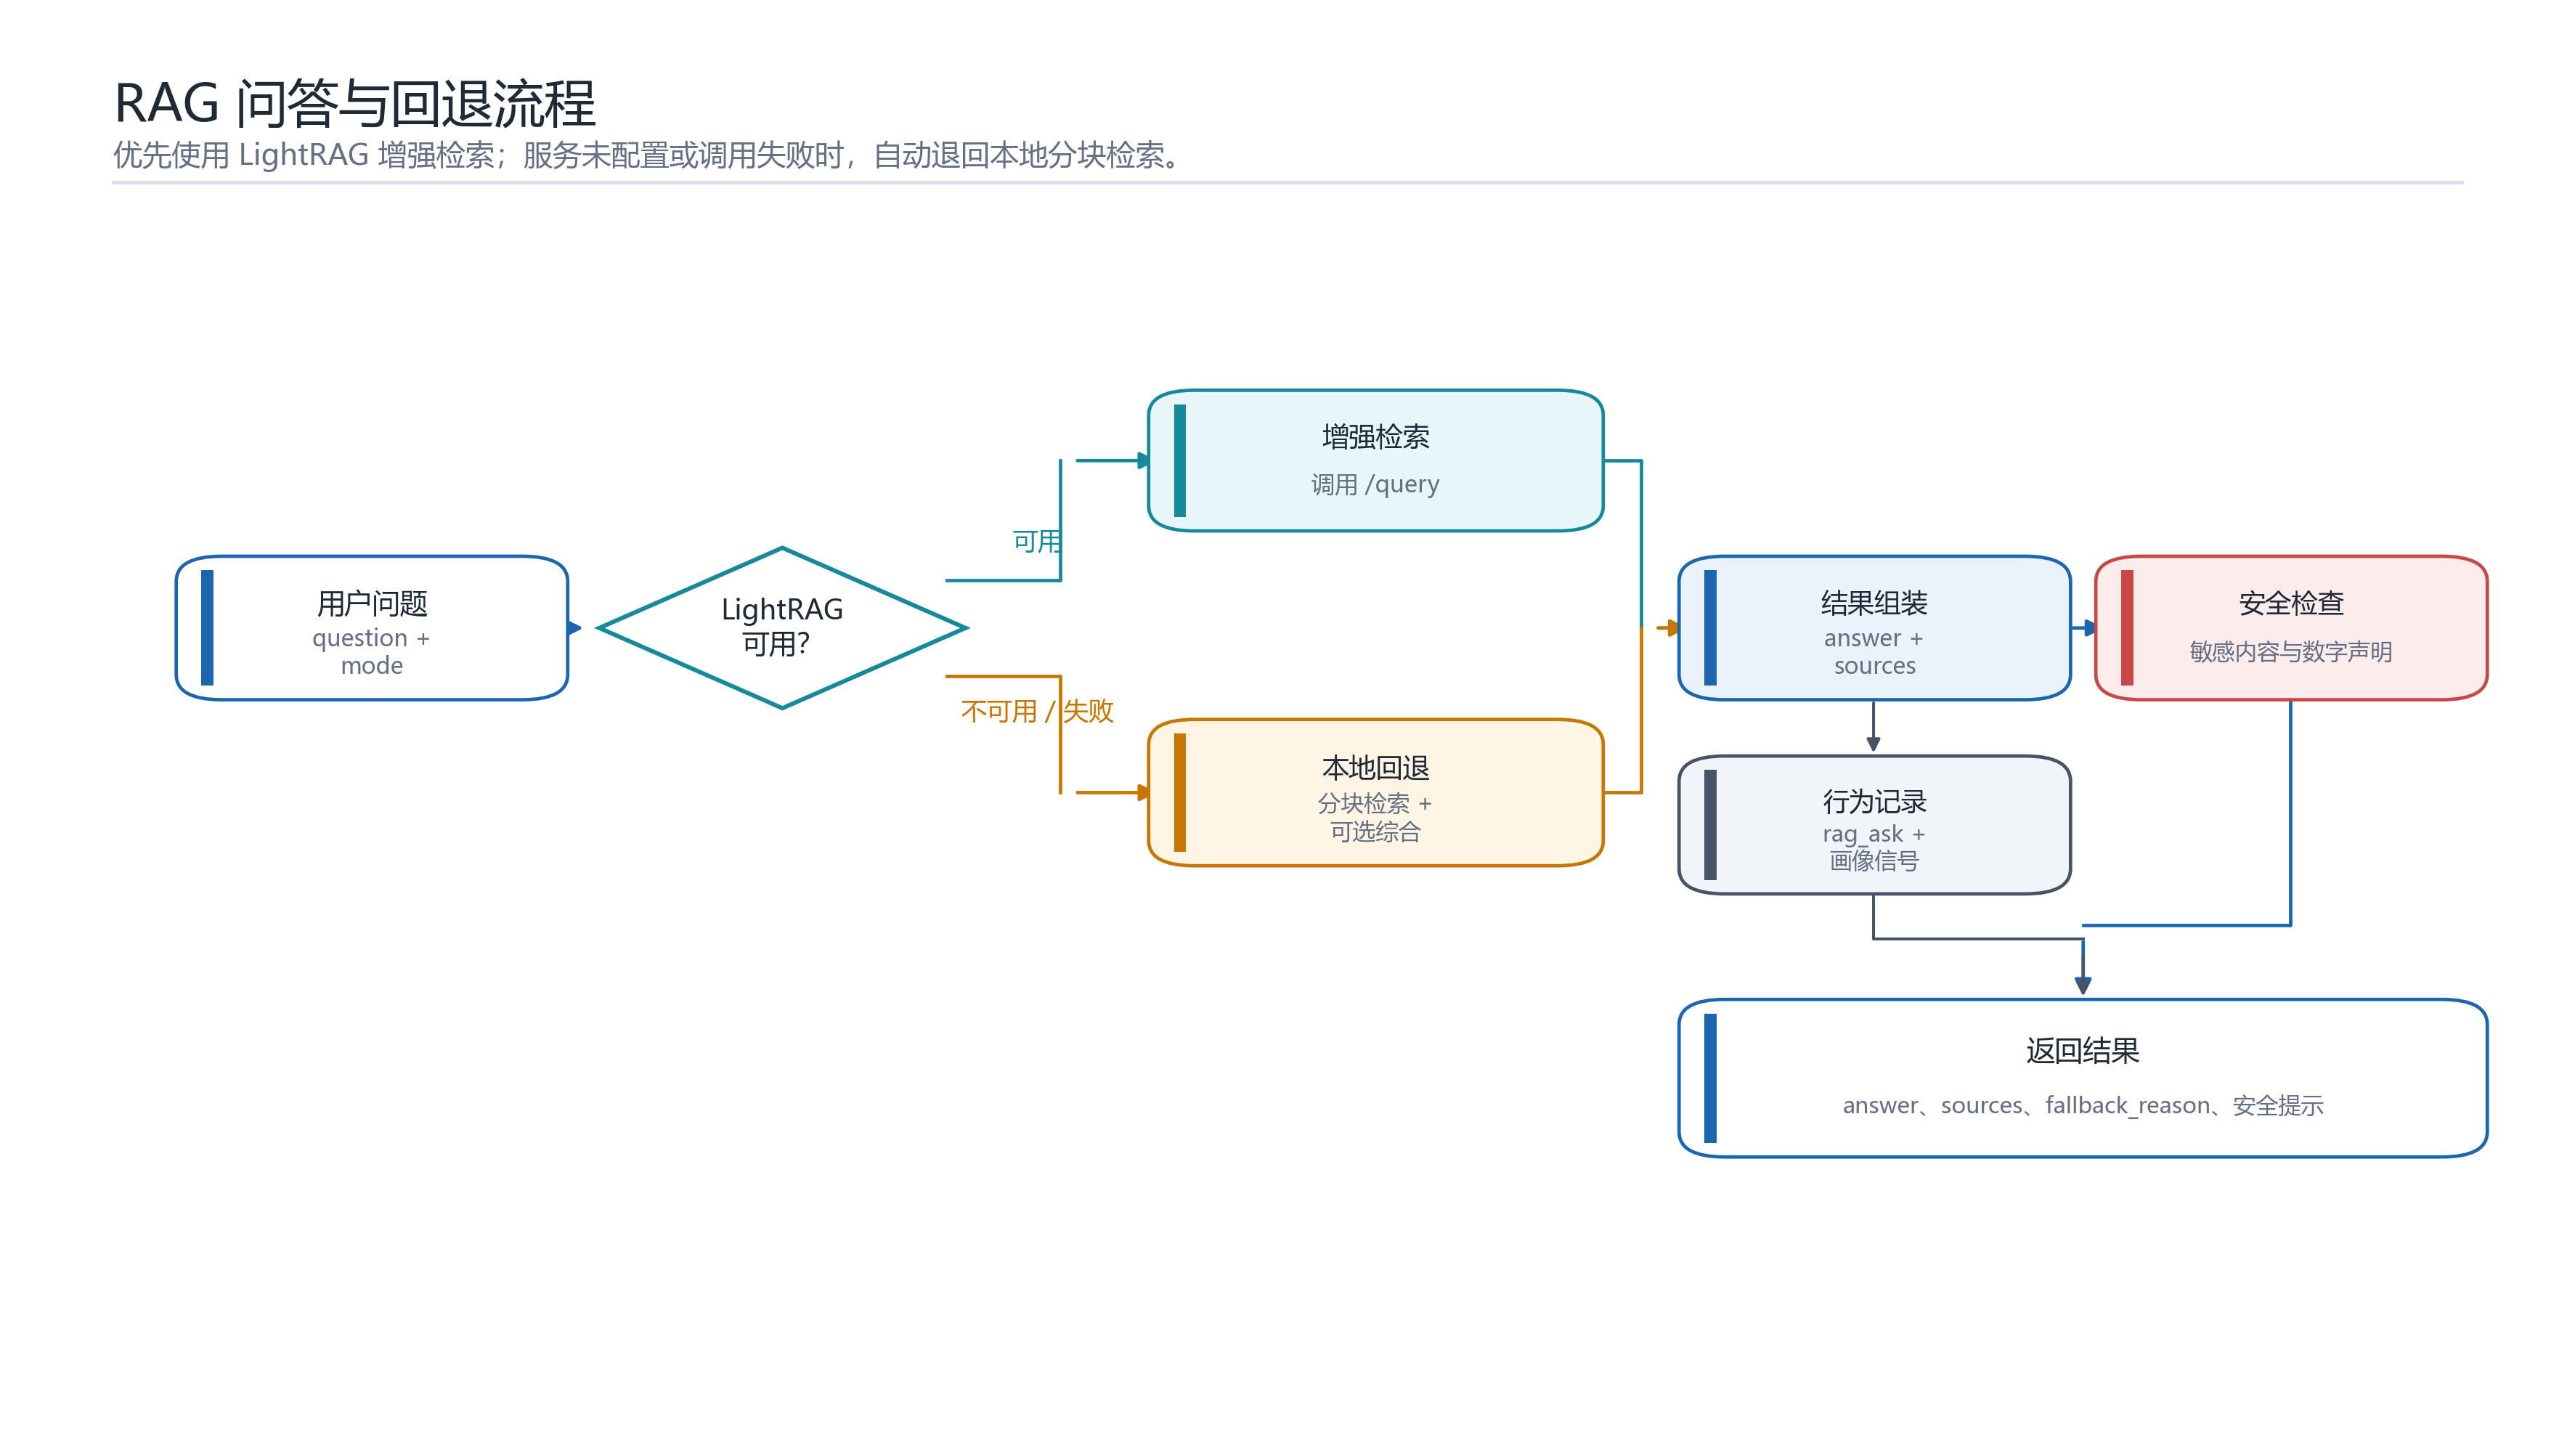
\includegraphics[width=0.95\textwidth]{fig_rag_flow.png}
  \caption{RAG 问答与回退流程图}
\end{figure}

RAG 问答设计包含主路径与回退路径：
\begin{enumerate}
  \item 用户在知识问答页签输入问题并选择 RAG 模式。
  \item 后端检查 \texttt{LIGHTRAG\_BASE\_URL} 是否配置。
  \item 若 LightRAG 可用，系统调用其 \texttt{/query} 接口返回增强检索答案。
  \item 若 LightRAG 未配置或调用失败，系统对当前课程的 Markdown 和 PDF 文本构建本地分块索引，按词法相似度检索相关片段。
  \item 若 \texttt{rag\_tutor} 路由可用，系统使用 LLM 基于检索片段综合回答；否则返回抽取式片段。
  \item 输出经过安全检查后返回前端，并记录 \texttt{rag\_ask} 行为事件。
\end{enumerate}

该流程的核心目标不是保证所有问答都依赖外部知识库，而是在“增强检索效果”和“本地可用性”之间取得平衡。LightRAG 路径适合已完成索引的课程资料，可利用外部服务维护的文档关系和检索能力；本地回退路径则面向离线和服务异常场景，至少保证用户可以围绕当前课程文件获得片段级回答。前端在展示答案时应同时呈现检索模式、来源文件和回退提示，使用户能够判断答案的可信边界。

\chapter{模块设计}

\section{功能模块划分}

\begin{figure}[H]
  \centering
  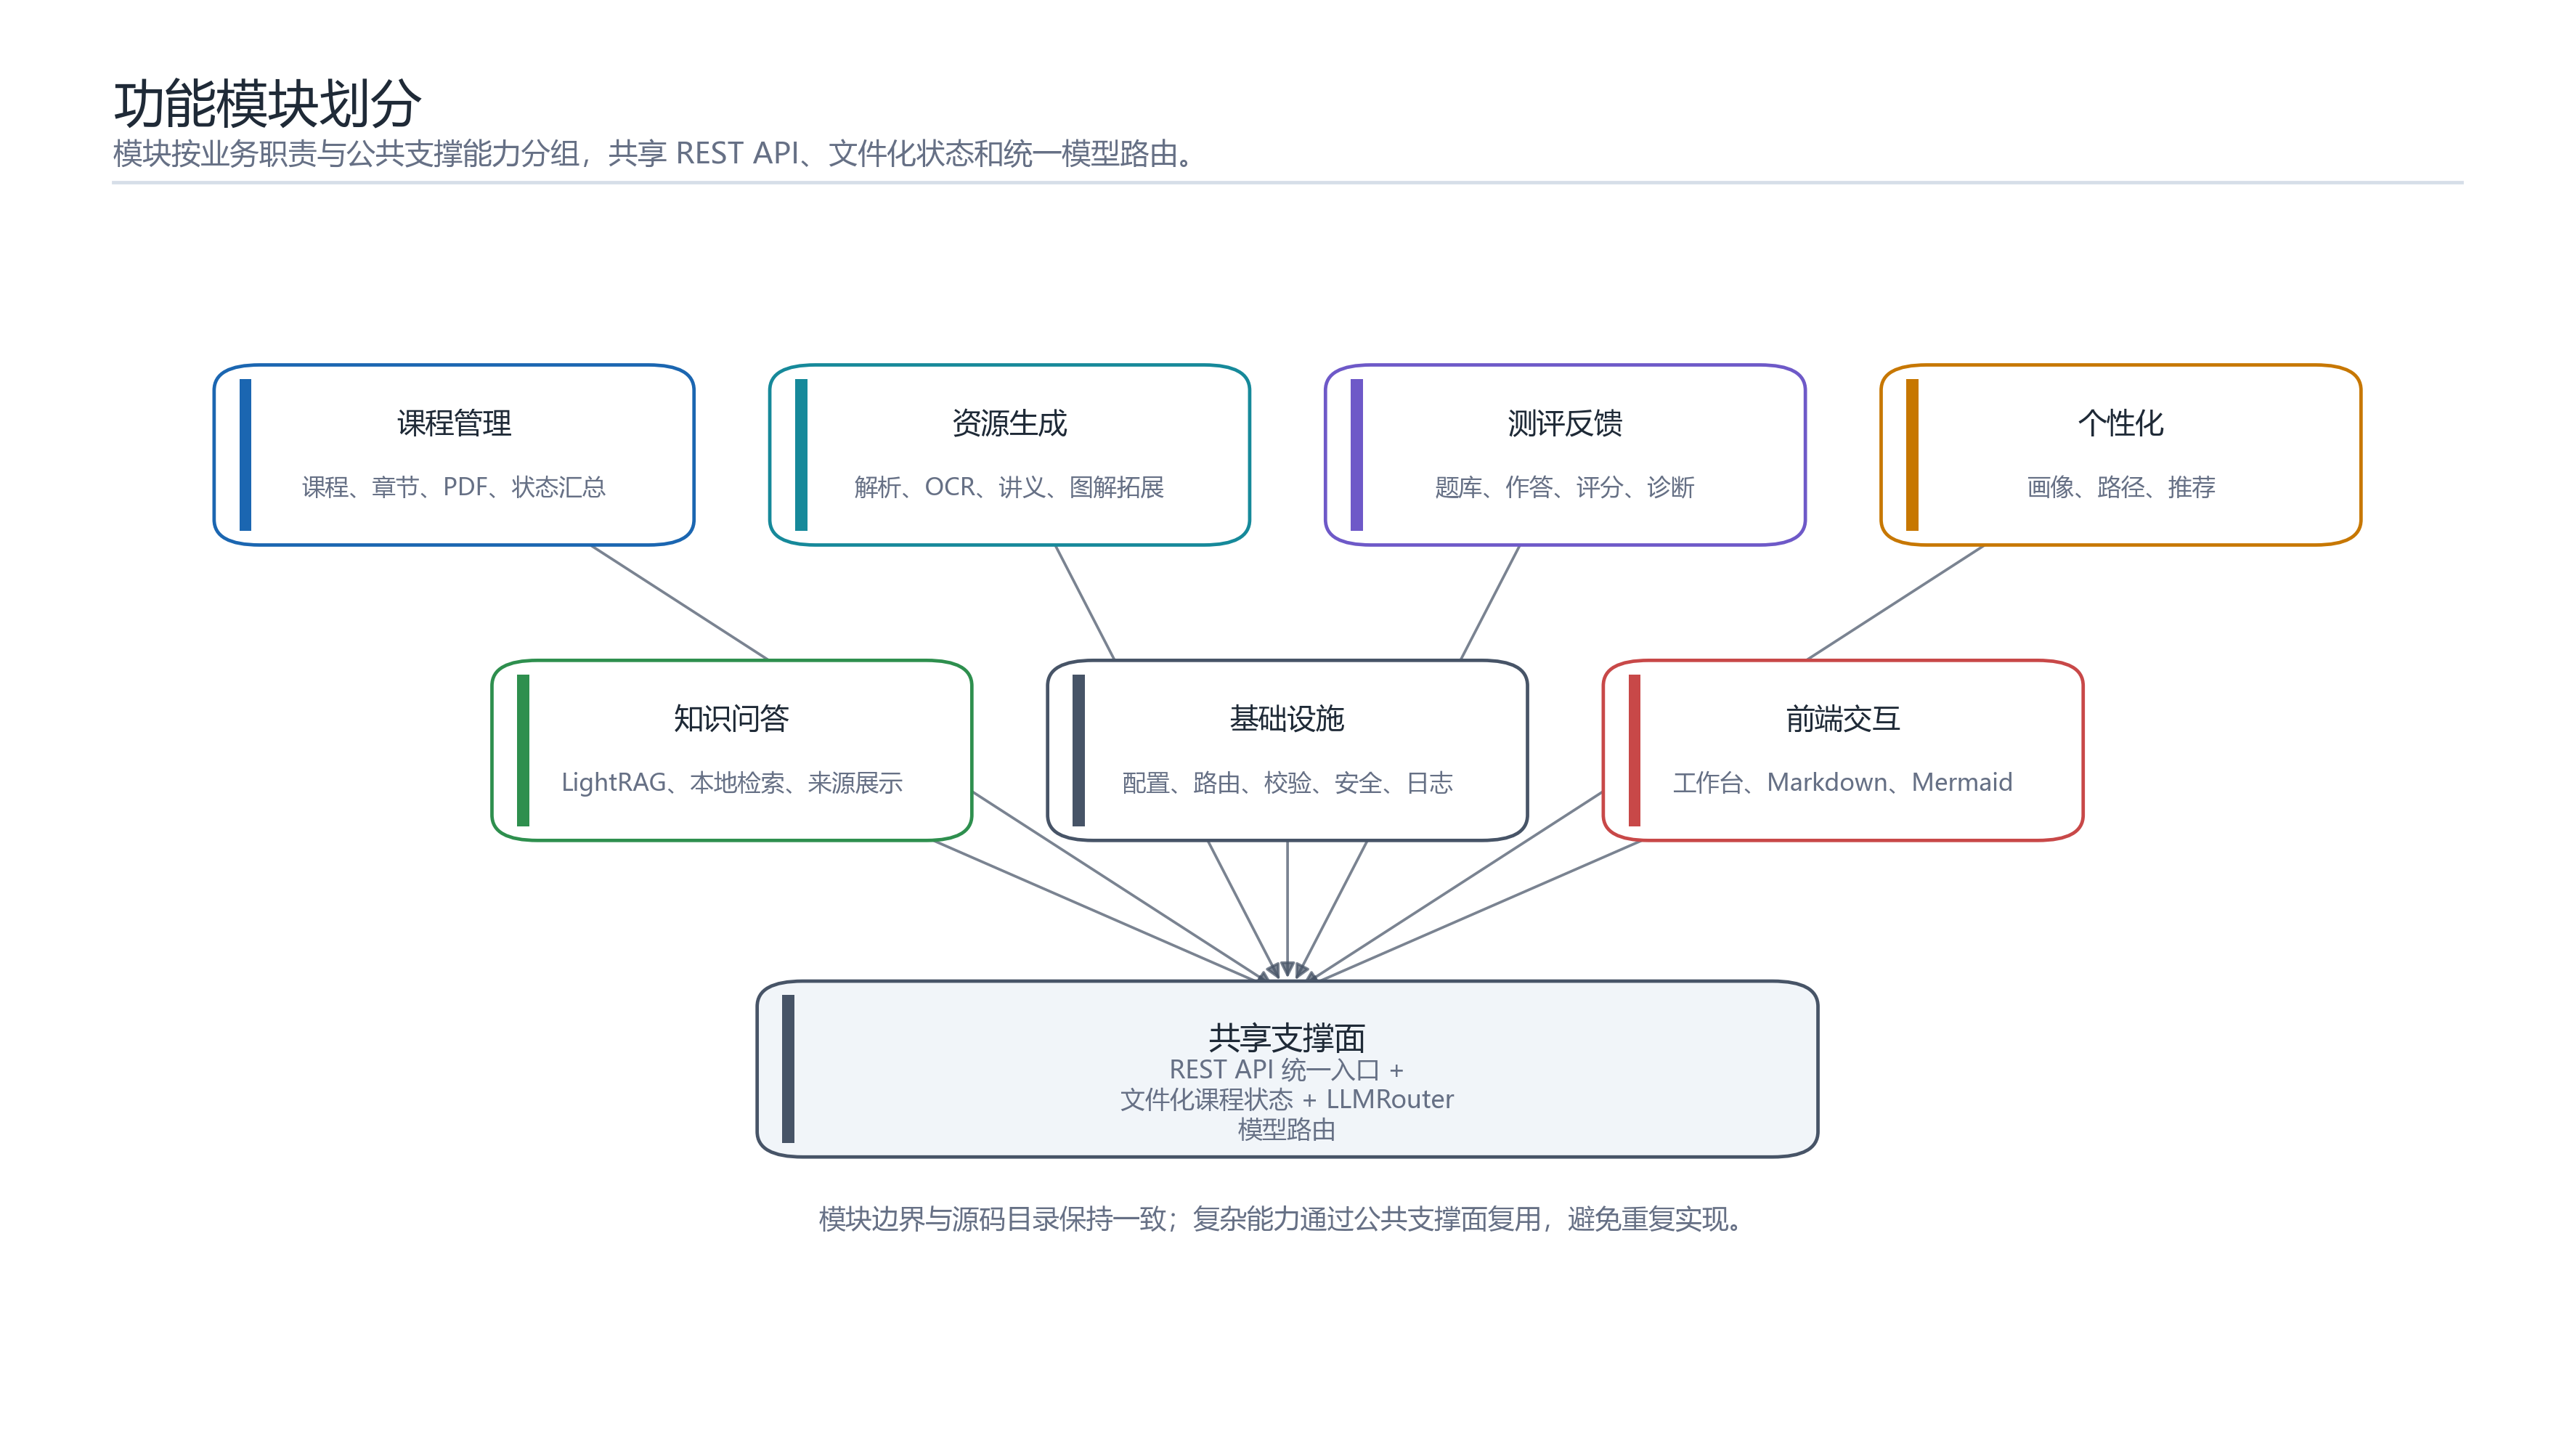
\includegraphics[width=0.98\textwidth]{fig_module_structure.png}
  \caption{功能模块划分图}
\end{figure}

\section{前端模块}

前端位于 \texttt{webapp/static}，主要由 \texttt{index.html}、\texttt{style.css} 和 \texttt{app.js} 组成。前端不依赖复杂构建链，适合本地运行和快速部署。

\begin{longtable}{p{0.25\textwidth}p{0.63\textwidth}}
\toprule
前端区域 & 职责\\
\midrule
课程驾驶舱 & 课程选择、新建、改名、删除，章节列表展示与章节操作入口。\\
资料接入区 & PDF 选择或拖拽上传，触发 \texttt{/api/upload}。\\
资源中心 & 获取并渲染 Markdown 文件，支持 Mermaid 图表渲染和缩放。\\
智能测评页签 & 读取 \texttt{Quiz.json}，渲染题目，执行客观题客户端检查，提交答案到后端。\\
知识问答页签 & 输入课程问题、选择 LightRAG 模式、触发索引与问答请求。\\
学习画像页签 & 表单编辑画像、提交访谈记录、生成路径、预览画像和学习计划。\\
提示与状态组件 & 展示模型接口、检索模式、错误提示、推荐下一步和操作反馈。\\
\bottomrule
\end{longtable}

\section{后端模块}

后端以 \texttt{webapp/server.py} 为 HTTP 接口层，配合 \texttt{main.py} 提供 CLI 入口。核心模块如下：

\begin{longtable}{p{0.24\textwidth}p{0.20\textwidth}p{0.45\textwidth}}
\toprule
模块 & 文件 & 主要职责\\
\midrule
入口编排 & \texttt{main.py} & 解析 CLI 命令，加载配置，创建 LLMRouter，调用对应智能体。\\
Web 服务 & \texttt{webapp/server.py} & FastAPI 路由、上传、状态聚合、长任务调度、RAG 问答和静态文件服务。\\
配置加载 & \texttt{core/config.py} & 合并 \texttt{.env} 与 \texttt{config.yaml}，解析每个智能体的模型路由。\\
模型路由 & \texttt{core/llm\_router.py} & 对接 Anthropic、OpenAI、vLLM、Ollama，统一聊天接口和错误提示。\\
课程库 & \texttt{core/library.py} & 管理课程、章节、PDF、元数据、章节状态和迁移逻辑。\\
PDF/OCR & \texttt{core/pdf\_parser.py}、\texttt{core/ocr.py} & PDF 文本提取、页面渲染、OCR 可用性检查和图片识别。\\
画像存储 & \texttt{core/personalization.py} & 画像 JSON 合并、Markdown 渲染、自动信号追加。\\
RAG 客户端 & \texttt{core/rag\_client.py} & LightRAG REST 调用、本地分块检索、抽取式或 LLM 综合回答。\\
安全检查 & \texttt{core/safety.py} & 检测敏感内容、未溯源数字声明并生成安全提示。\\
行为日志 & \texttt{core/telemetry.py} & 记录 JSONL 行为事件，生成行为摘要。\\
推荐模块 & \texttt{core/recommendations.py} & 根据课程状态、画像和事件生成下一步推荐。\\
\bottomrule
\end{longtable}

\section{智能体模块}

\begin{figure}[H]
  \centering
  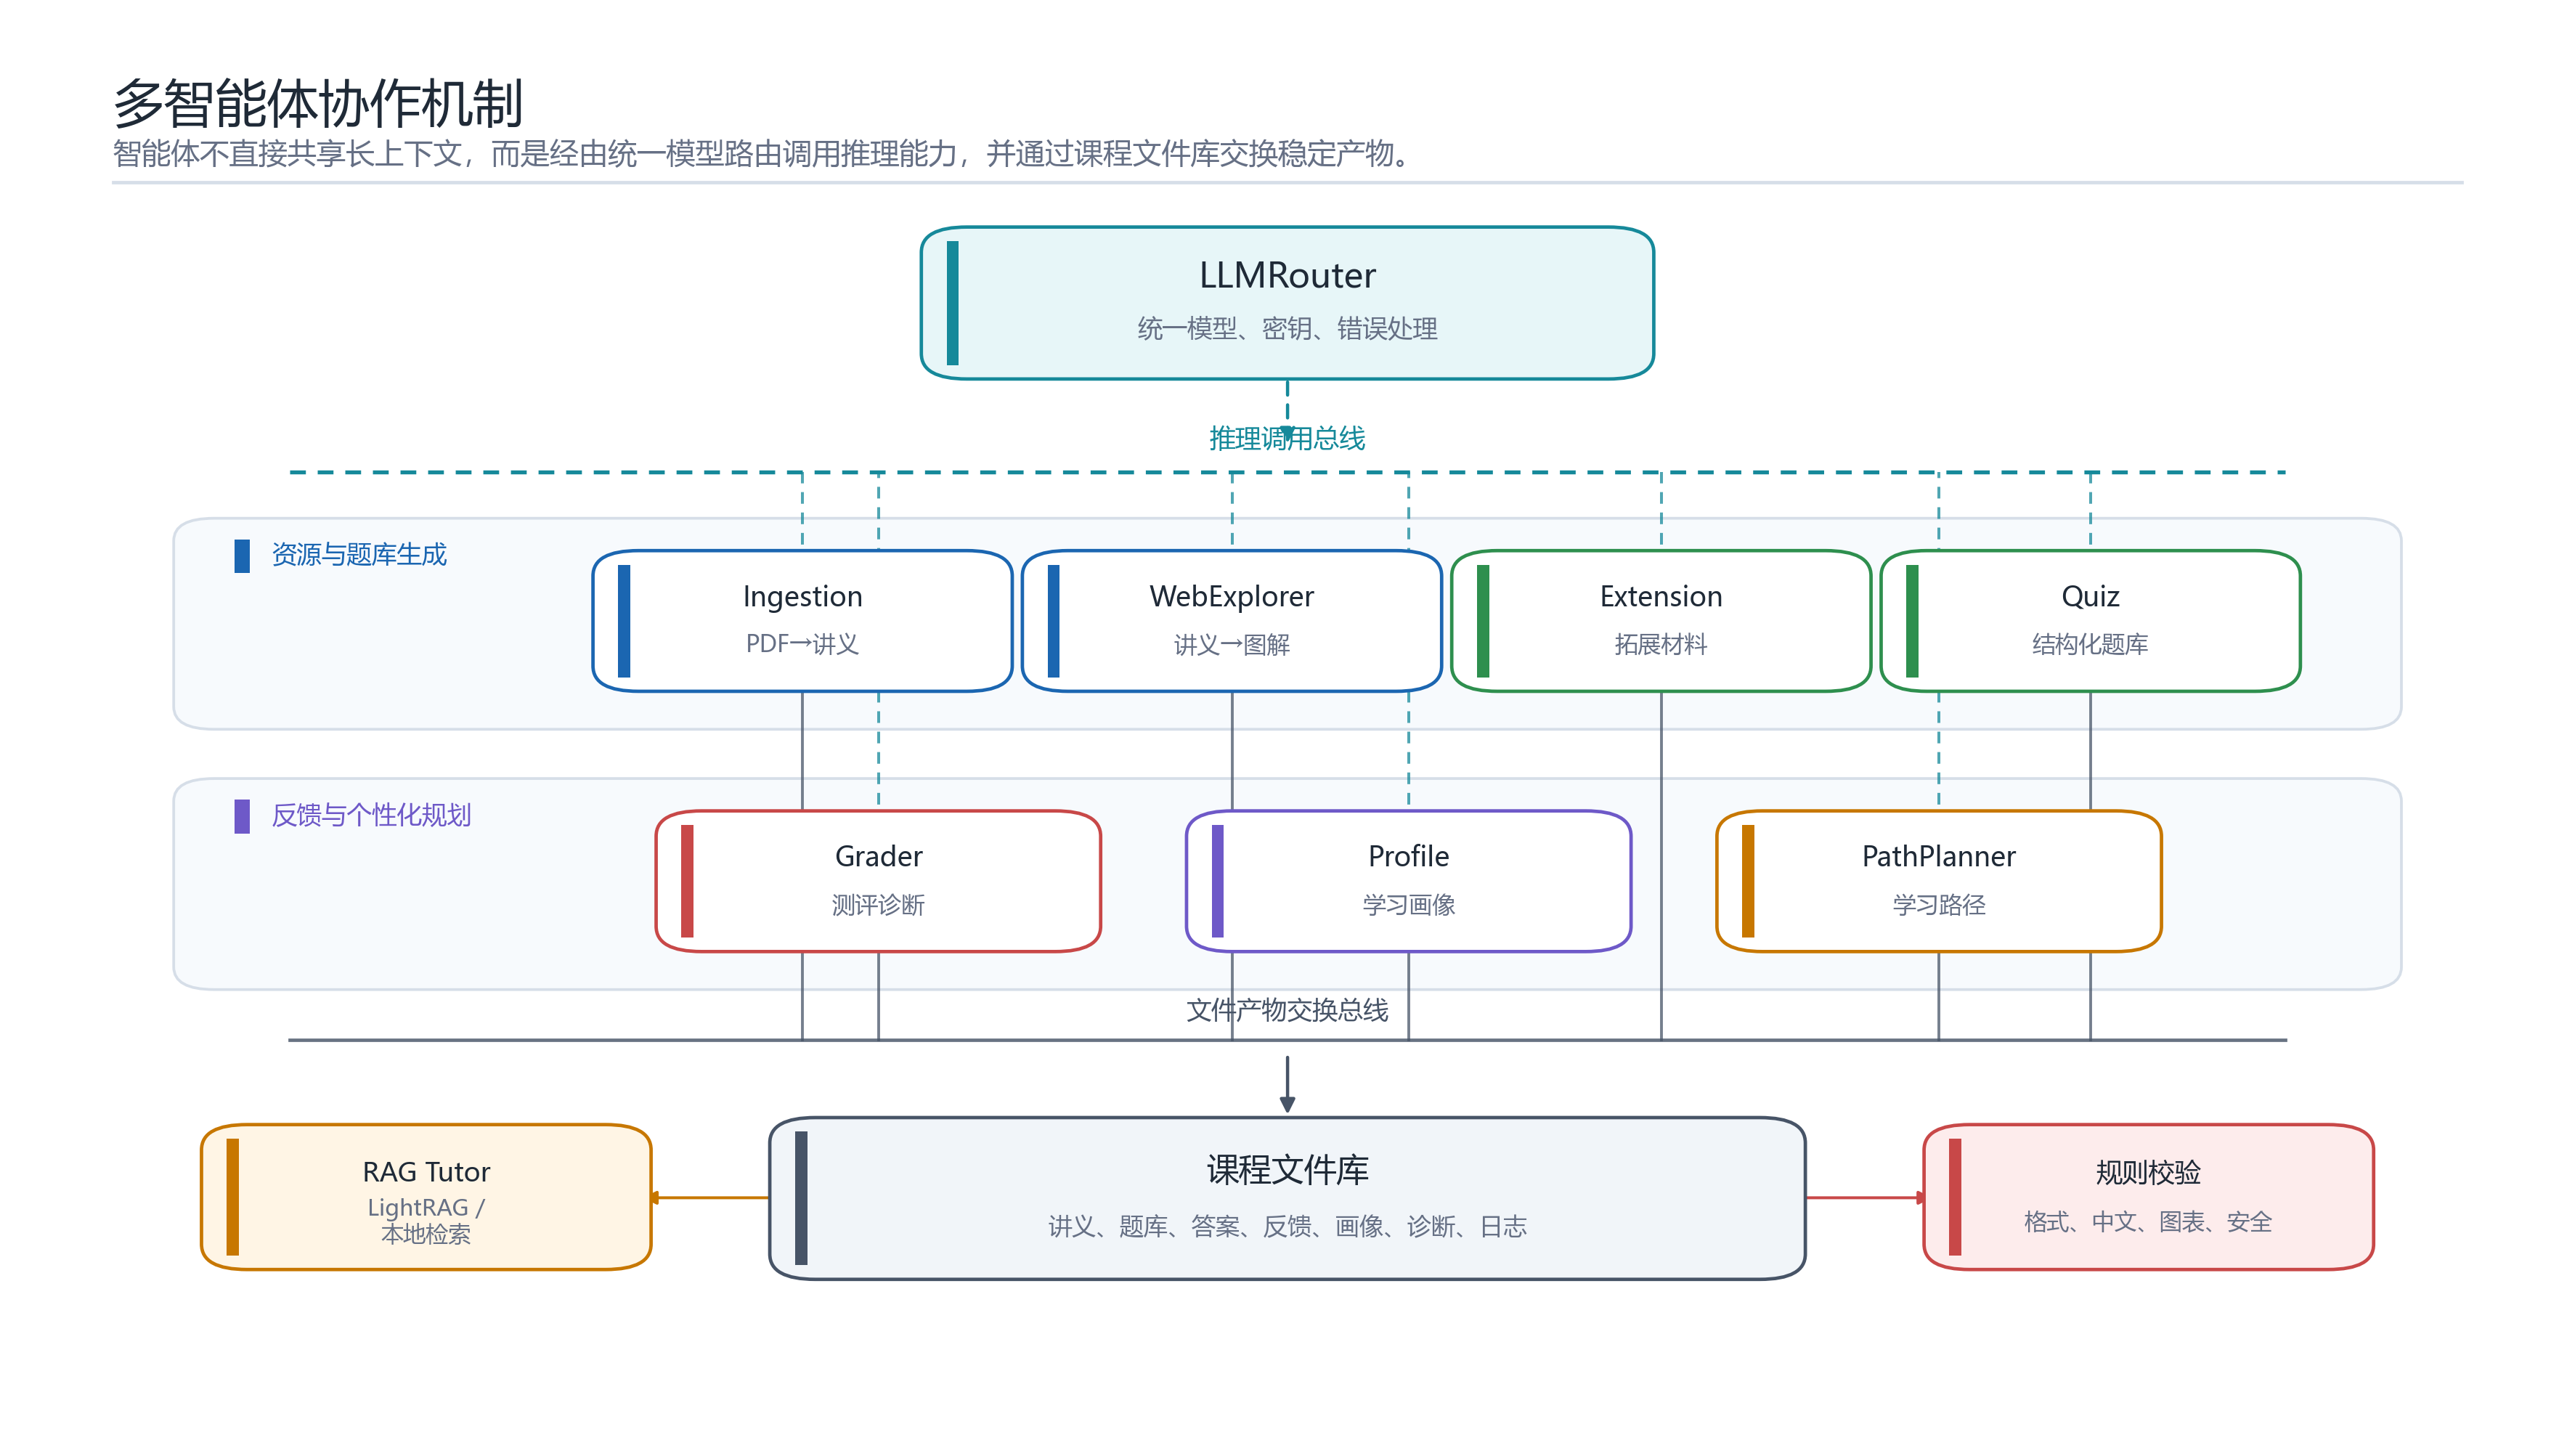
\includegraphics[width=0.96\textwidth]{fig_agent_collaboration.png}
  \caption{多智能体协作关系图}
\end{figure}

\begin{longtable}{p{0.22\textwidth}p{0.22\textwidth}p{0.45\textwidth}}
\toprule
智能体 & 文件 & 设计说明\\
\midrule
Ingestion Agent & \texttt{agents/ingestion\_agent.py} & 读取 PDF 解析结果，按基础、应用、提升三层生成中文讲义，使用合成规则校验器。\\
WebExplorer & \texttt{agents/web\_explorer.py} & 根据讲义提取概念并生成 Mermaid 知识结构图，当前实现不联网抓图。\\
Extension Agent & \texttt{agents/extension\_agent.py} & 基于讲义和图解生成拓展学习材料，并进行安全检查。\\
Quiz Agent & \texttt{agents/quiz\_agent.py} & 生成结构化测评 JSON，渲染题面和作答模板，校验题型和数量。\\
Grader Agent & \texttt{agents/grader\_agent.py} & 读取题目与答案，生成诊断式反馈，抽取学习缺口写入诊断记录。\\
Profile Agent & \texttt{agents/profile\_agent.py} & 结合访谈、诊断和章节状态生成学生画像 JSON。\\
Path Planner & \texttt{agents/path\_planner.py} & 基于画像、诊断和学习进度生成个性化学习路径。\\
\bottomrule
\end{longtable}

\section{核心公共机制}

\subsection{统一模型路由}

\texttt{config.yaml} 中把模型调用拆成逻辑引擎和具体模型。智能体只读取自己的路由，不直接保存 API Key 或服务地址。逻辑引擎 \texttt{api} 会根据 \texttt{API\_PROVIDER} 解析为 \texttt{anthropic}、\texttt{openai} 或 \texttt{vllm}；本地对话类能力可走 \texttt{ollama}。

这种设计使模型替换集中在配置层完成。例如要将资料解析智能体从 OpenAI 切换到自部署 vLLM，只需要修改 \texttt{.env} 中的 \texttt{API\_PROVIDER} 和 \texttt{VLLM\_BASE\_URL}，无需改动各智能体代码。

\subsection{规则校验与有限重试}

\texttt{BaseAgent.run\_validated} 在生成后执行校验器。若校验失败，系统把失败原因追加到对话中，要求模型重写完整响应。当前合成讲义校验包括：
\begin{itemize}
  \item 中文内容应保持 UTF-8 可读，不出现乱码、韩文字形或非预期外文片段。
  \item 至少包含一个 Mermaid 图块。
  \item 示例导入应出现在抽象知识、定义或原理说明之前。
\end{itemize}

测评和反馈模块也包含 JSON 结构、题型、数量和非二元化反馈等校验。

\subsection{文件化共享状态}

系统使用文件作为智能体之间的共享状态，避免在编排层传递长上下文。章节级资料和课程级状态均可以被用户直接查看，也可以被其他智能体读取。

\begin{figure}[H]
  \centering
  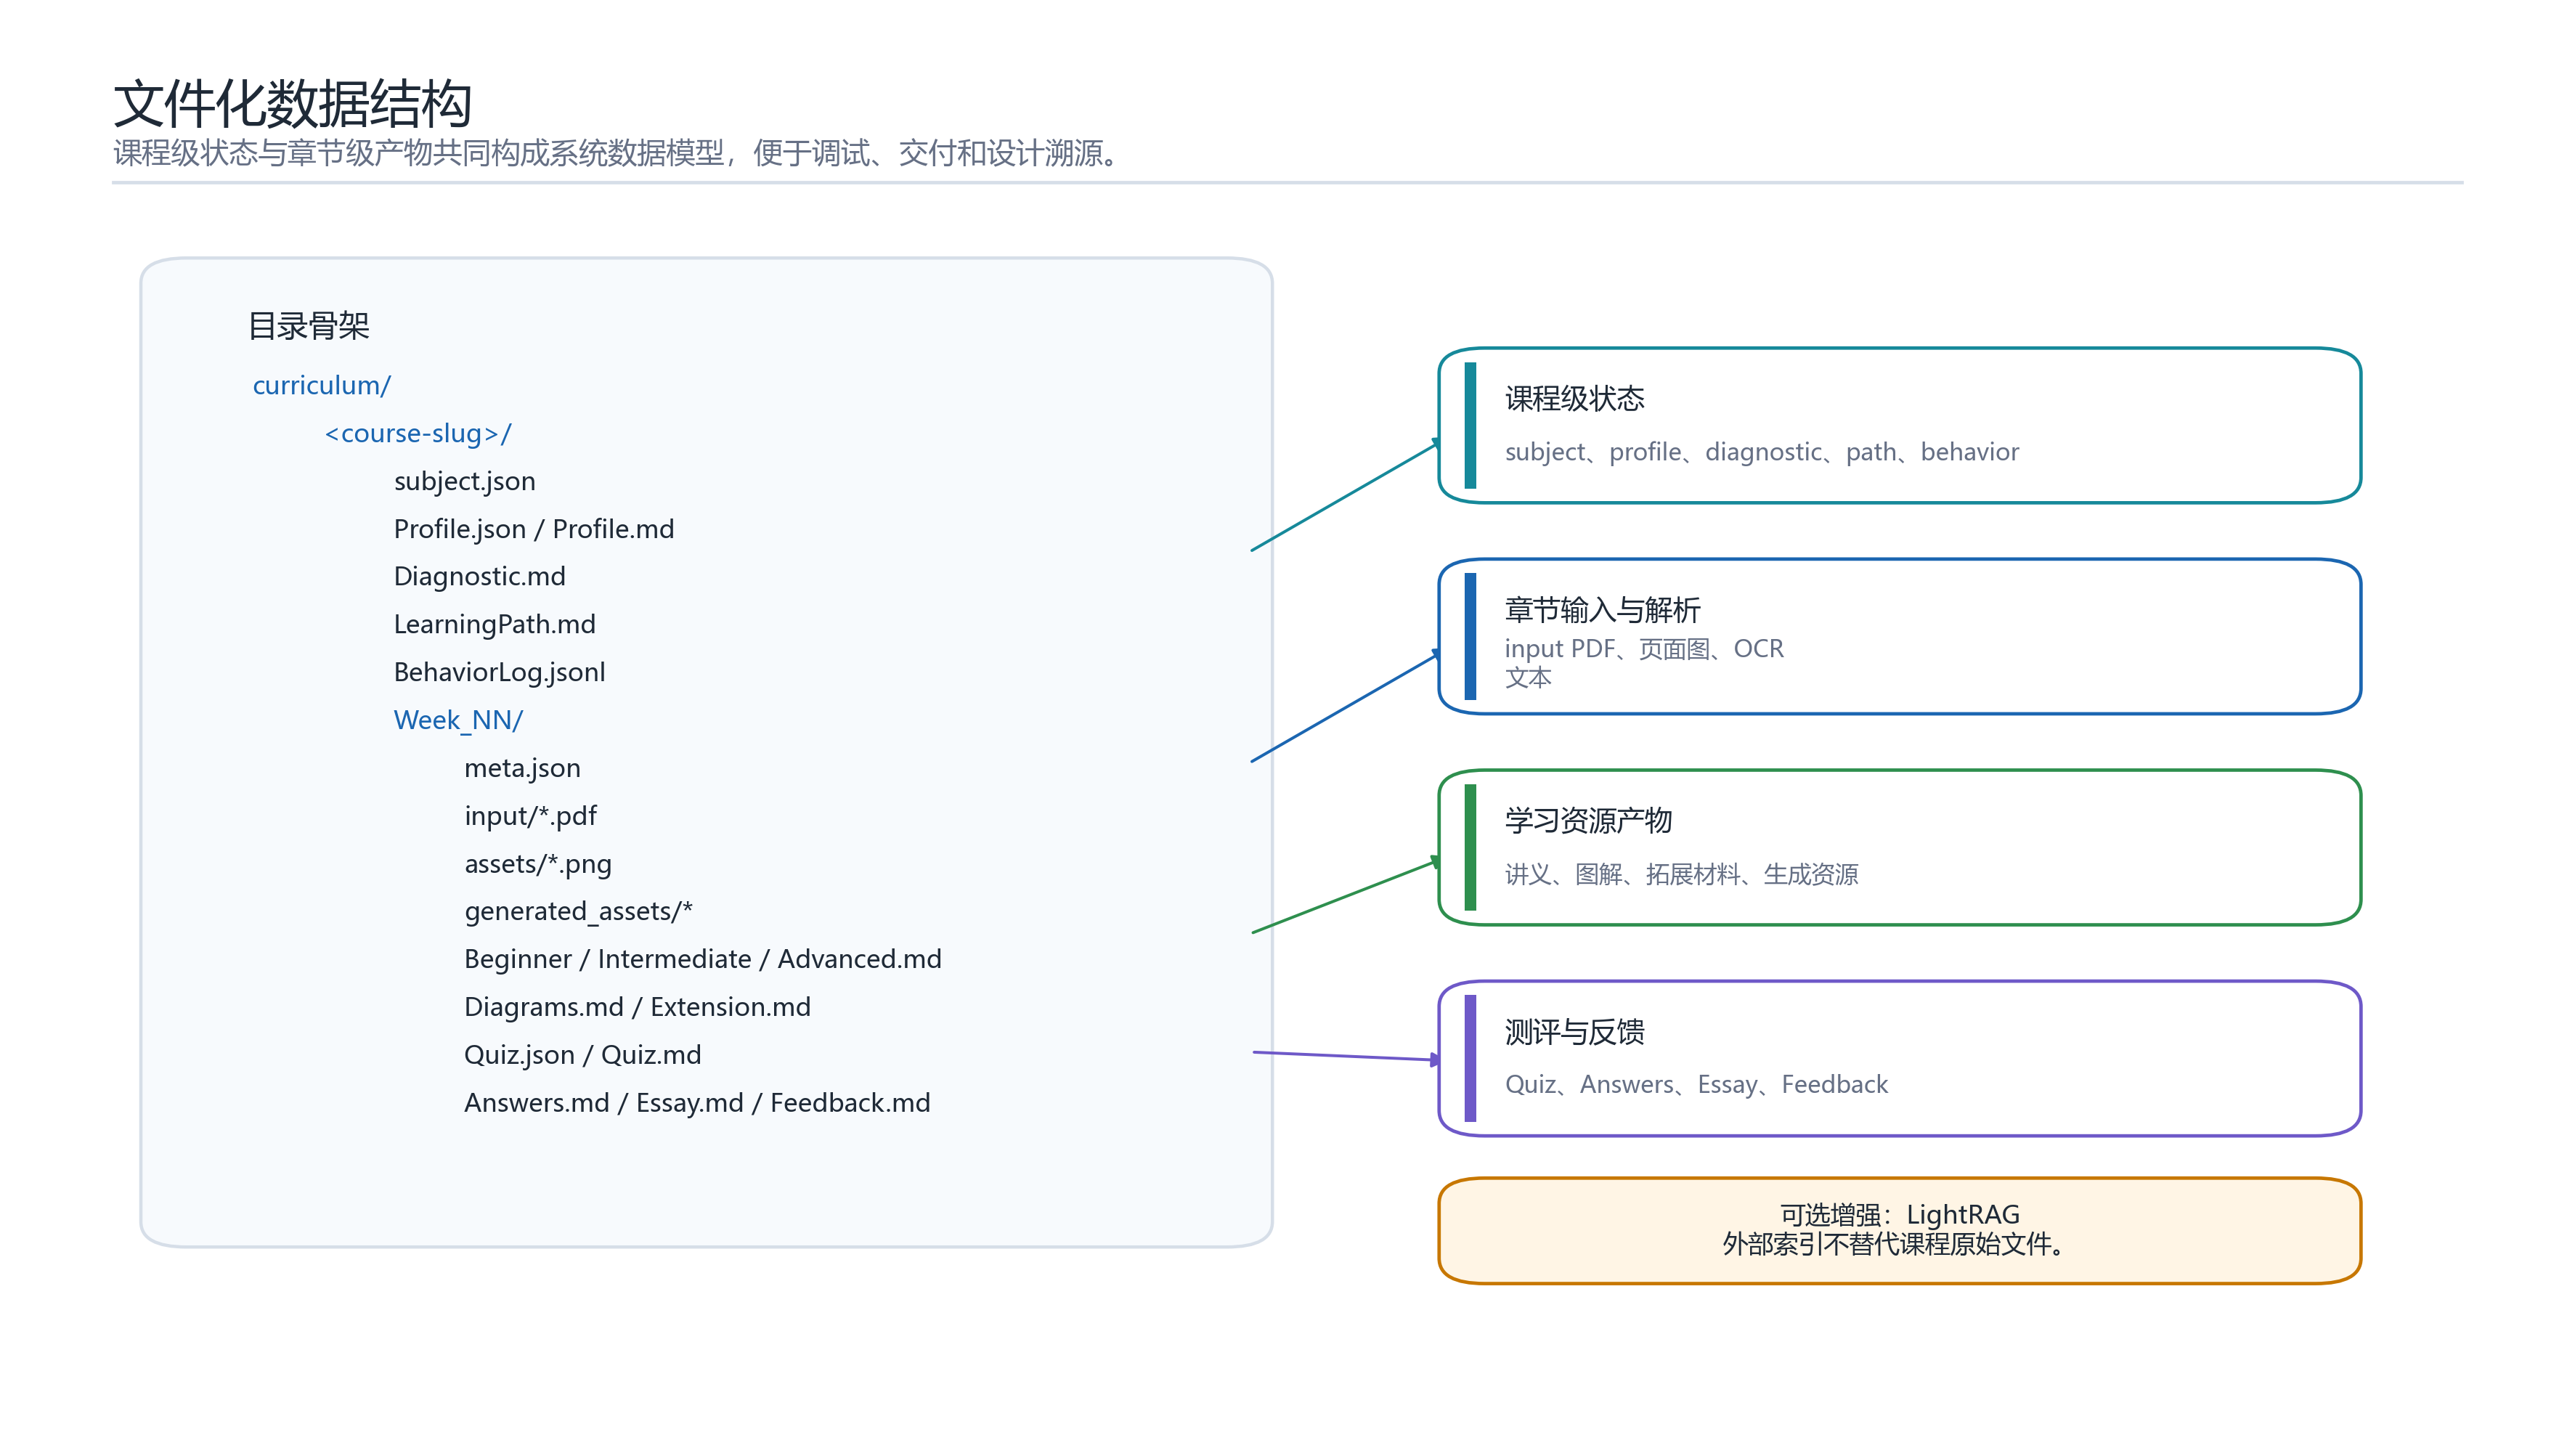
\includegraphics[width=0.90\textwidth]{fig_filesystem_data_model.png}
  \caption{文件化数据结构图}
\end{figure}

\chapter{接口设计}

\section{内部接口}

系统内部接口包括 Python 类接口和 HTTP API 两类。Python 类接口主要用于 CLI 和 Web 层复用同一套智能体；HTTP API 主要服务前端页面。

\subsection{课程与状态接口}

\begin{longtable}{p{0.24\textwidth}p{0.18\textwidth}p{0.45\textwidth}}
\toprule
接口 & 方法 & 功能说明\\
\midrule
\texttt{/api/state} & GET & 返回课程列表、当前课程、章节状态、模型提供方、RAG 状态和推荐下一步。\\
\texttt{/api/subject/create} & POST & 创建课程，写入 \texttt{subject.json}。\\
\texttt{/api/subject/select} & POST & 设置当前活动课程。\\
\texttt{/api/subject/rename} & POST & 修改课程显示名称，课程 slug 保持不变。\\
\texttt{/api/subject/delete} & POST & 删除课程目录或标记为已删除。\\
\texttt{/api/diagnostic} & GET & 返回当前课程的 \texttt{Diagnostic.md} 内容。\\
\texttt{/api/behavior} & GET/POST & 读取行为摘要或记录行为事件。\\
\bottomrule
\end{longtable}

\subsection{章节文件接口}

\begin{longtable}{p{0.24\textwidth}p{0.18\textwidth}p{0.45\textwidth}}
\toprule
接口 & 方法 & 功能说明\\
\midrule
\texttt{/api/upload} & POST & 上传 PDF 到新章节或指定章节的 \texttt{input} 目录。\\
\texttt{/api/week/\{week\}/file/\{name\}} & GET & 读取章节下指定 Markdown 或文本文件。\\
\texttt{/api/week/\{week\}/asset/\{name\}} & GET & 读取章节 \texttt{assets} 下的图片文件。\\
\texttt{/api/week/\{week\}/generated/\{name\}} & GET & 读取章节 \texttt{generated\_assets} 下的生成资源。\\
\texttt{/api/save} & POST & 保存用户可写文件，目前仅允许 \texttt{Answers.md} 和 \texttt{Essay.md}。\\
\bottomrule
\end{longtable}

文件读取接口通过 \texttt{\_safe\_name} 禁止文件名包含路径分隔符或 \texttt{..}，避免路径穿越。

\subsection{资源生成接口}

\begin{longtable}{p{0.24\textwidth}p{0.18\textwidth}p{0.45\textwidth}}
\toprule
接口 & 方法 & 功能说明\\
\midrule
\texttt{/api/ingest} & POST & 调用资料解析智能体生成三层讲义。\\
\texttt{/api/ingest/stream} & GET & 通过 SSE 返回资料解析和讲义生成进度。\\
\texttt{/api/explore} & POST & 生成知识图解 \texttt{Diagrams.md}。\\
\texttt{/api/extension} & POST & 生成拓展学习材料 \texttt{Extension.md}。\\
\texttt{/api/quiz} & POST & 生成结构化题库和作答模板。\\
\texttt{/api/grade} & POST & 生成深度诊断反馈并追加诊断发现。\\
\bottomrule
\end{longtable}

\subsection{画像、路径与 RAG 接口}

\begin{longtable}{p{0.24\textwidth}p{0.18\textwidth}p{0.45\textwidth}}
\toprule
接口 & 方法 & 功能说明\\
\midrule
\texttt{/api/profile} & GET & 读取画像 JSON 和 Markdown。\\
\texttt{/api/profile/save} & POST & 保存用户编辑的画像。\\
\texttt{/api/profile/build} & POST & 根据访谈记录、诊断和章节状态生成画像。\\
\texttt{/api/path} & POST & 生成个性化学习路径。\\
\texttt{/api/path} & GET & 读取 \texttt{LearningPath.md}。\\
\texttt{/api/rag/ask} & POST & 课程资料问答，优先 LightRAG，失败则本地检索回退。\\
\texttt{/api/rag/status} & GET & 返回 LightRAG 文档处理状态。\\
\texttt{/api/rag/index-week} & POST & 将当前课程全部可索引资料上传至 LightRAG。\\
\texttt{/api/safety/check} & POST & 对指定文本执行安全检查。\\
\bottomrule
\end{longtable}

\section{外部接口}

\begin{longtable}{p{0.23\textwidth}p{0.60\textwidth}}
\toprule
外部服务 & 用途\\
\midrule
OpenAI API & 可作为主系统 \texttt{api} 引擎，执行讲义、题库、反馈、画像和路径生成。\\
Anthropic API & 可作为主系统 \texttt{api} 引擎的另一种云模型提供方。\\
OpenAI-compatible vLLM & 可接入自部署模型服务，适合本地或服务器推理环境。\\
Ollama & 可作为本地模型服务，适合低延迟本地对话或辅助生成。\\
LightRAG Server & 提供知识图谱增强检索、文档上传、文档处理状态查询和问答。\\
Tesseract OCR & 对扫描版或图片型 PDF 页面执行 OCR 识别。\\
\bottomrule
\end{longtable}

\chapter{运行设计}

\section{运行模块交互}

系统启动后，\texttt{main.py} 加载配置并构造 \texttt{settings} 和 \texttt{router}。当执行 \texttt{serve} 命令时，Uvicorn 启动 FastAPI 应用；用户在浏览器中触发操作后，前端调用 HTTP API，后端根据具体请求读取文件、调用智能体或调用 RAG 客户端。

对于讲义生成、题库生成、评分等耗时任务，后端使用 \texttt{asyncio.to\_thread} 将同步模型调用放入工作线程，避免阻塞事件循环。对于资料解析任务，系统还提供 \texttt{/api/ingest/stream}，通过 Server-Sent Events 返回“正在解析 PDF”“正在生成基础讲义”等进度事件。

这种运行方式符合本地学习工作台的特点：轻量查询接口保持即时响应，长任务通过前端状态提示降低等待不确定性，模型服务异常则以结构化错误返回给用户。若系统扩展为多人课程平台，可将当前线程级长任务迁移到后台任务队列，并用数据库记录任务状态和执行日志。

\section{运行控制}

\subsection{主系统启动}

\begin{lstlisting}[language=bash]
cd E:\pythonproject\agent\agent\agentic-study-system
python main.py serve --port 8000
\end{lstlisting}

\subsection{命令行运行}

系统保留 CLI 入口，便于测试和自动化运行：
\begin{lstlisting}[language=bash]
python main.py ingest    --week 1 --subject course-slug
python main.py explore   --week 1 --subject course-slug
python main.py extension --week 1 --subject course-slug
python main.py quiz      --week 1 --subject course-slug
python main.py grade     --week 1 --subject course-slug
\end{lstlisting}

\subsection{LightRAG 启动}

LightRAG 是可选增强服务。项目提供 PowerShell 启动脚本：
\begin{lstlisting}[language=bash]
.\scripts\start_lightrag.ps1
\end{lstlisting}

主系统通过 \texttt{LIGHTRAG\_BASE\_URL} 调用 LightRAG；若未配置或失败，问答功能自动走本地检索。

\section{部署方案}

本项目适合以下部署方式：
\begin{enumerate}
  \item 本地单机部署。开发机安装 Python 依赖、配置 \texttt{.env}，直接启动主系统。
  \item 本地主系统 + 外部模型服务。主系统本地运行，模型调用走 OpenAI、Anthropic 或远程 vLLM。
  \item 本地主系统 + 本地 LightRAG/Ollama。适合构建“资料索引 + 检索增强问答 + 本地推理”的完整闭环。
\end{enumerate}

\chapter{界面设计}

\section{整体布局}

系统界面采用单页学习工作台结构，左侧为课程和章节操作，右侧为资源中心、测评、问答、画像和诊断。该结构可以减少页面跳转，让用户围绕当前课程完成从资料接入到反馈追踪的完整流程。

\begin{longtable}{p{0.24\textwidth}p{0.62\textwidth}}
\toprule
界面区域 & 设计说明\\
\midrule
课程驾驶舱 & 提供课程选择、新建、重命名、删除、PDF 上传和章节流程管理，是系统的主要入口。\\
章节流程区 & 按章节展示资料接入、讲义生成、图解、拓展、测评和反馈状态，帮助用户判断当前学习单元进度。\\
资源中心 & 预览分层讲义、知识图解、拓展材料、反馈文件和生成资源，支持 Markdown 与 Mermaid 图表渲染。\\
智能测评 & 展示题库、客观题检查、开放题作答、综合论述保存和深度反馈入口。\\
知识问答 & 面向课程资料提问，支持检索模式选择、资料索引和来源展示。\\
学习画像 & 维护学生背景、学习目标、知识基础、短板、兴趣和资源偏好，并生成个性化学习路径。\\
学习诊断 & 展示课程级诊断日志，持续汇总测评反馈、薄弱点和概念缺口。\\
\bottomrule
\end{longtable}

\section{交互原则}

\begin{enumerate}
  \item 任务入口集中。与当前章节相关的生成操作集中在章节流程中，减少用户在多个页面之间寻找入口。
  \item 状态反馈明确。长任务执行时展示进度或等待提示；失败时显示可读错误信息和修复方向。
  \item 内容可追溯。讲义、题库、反馈、画像、路径和诊断均可在界面中打开对应 Markdown 或 JSON 产物。
  \item 中文优先。界面标签、提示信息、学习资源和诊断内容均以简体中文为主，降低学习使用门槛。
  \item 主次清晰。资料预览、题目作答、问答结果等核心内容保持较大阅读区域，辅助按钮和状态信息保持紧凑。
\end{enumerate}

\chapter{数据结构设计}

\section{逻辑结构设计}

系统以课程为最高层级，课程下包含多个章节，章节下保存输入资料、生成资源、测评与反馈文件。课程级状态用于持续追踪学习者画像、诊断和行为。

\begin{longtable}{p{0.22\textwidth}p{0.28\textwidth}p{0.38\textwidth}}
\toprule
逻辑对象 & 保存位置 & 说明\\
\midrule
课程 & \texttt{curriculum/<slug>} & 一门独立课程，包含名称、章节、画像和诊断。\\
章节 & \texttt{Week\_NN} & 一个学习单元，通常对应一次上传或一周课程内容。\\
课程资料 & \texttt{Week\_NN/input/*.pdf} & 用户上传的原始 PDF。\\
页面图片 & \texttt{Week\_NN/assets/*.png} & PDF 页面渲染图，供 OCR 或图像查看使用。\\
分层讲义 & \texttt{Beginner.md} 等 & 三层中文学习讲义。\\
测评题库 & \texttt{Quiz.json}/\texttt{Quiz.md} & 结构化题库和人类可读题面。\\
作答与反馈 & \texttt{Answers.md}/\texttt{Feedback.md} & 学生答案和诊断式反馈。\\
学习画像 & \texttt{Profile.json}/\texttt{Profile.md} & 结构化画像和 Markdown 预览。\\
学习路径 & \texttt{LearningPath.md} & 个性化路径规划结果。\\
行为日志 & \texttt{BehaviorLog.jsonl} & 追加式学习事件记录。\\
\bottomrule
\end{longtable}

\section{物理结构设计}

系统不依赖关系型数据库，主要使用文件系统保存状态。典型目录如下：

\begin{lstlisting}
agentic-study-system/
  curriculum/
    <course-slug>/
      subject.json
      Profile.json
      Profile.md
      Diagnostic.md
      LearningPath.md
      BehaviorLog.jsonl
      Week_01/
        meta.json
        input/
          *.pdf
        assets/
          *.png
        generated_assets/
        Beginner.md
        Intermediate.md
        Advanced.md
        Diagrams.md
        Extension.md
        Quiz.json
        Quiz.md
        Answers.md
        Essay.md
        Feedback.md
\end{lstlisting}

\section{主要数据文件设计}

\subsection{\texttt{subject.json}}

保存课程显示名称，课程目录 slug 不因重命名而改变。
\begin{lstlisting}
{
  "name": "人工智能导论"
}
\end{lstlisting}

\subsection{\texttt{Profile.json}}

学习画像包含基础信息、学习维度、状态与原始观察记录。
\begin{lstlisting}
{
  "basic": {
    "major": "",
    "grade": "",
    "target_course": "",
    "learning_goal": "",
    "time_budget": ""
  },
  "dimensions": {
    "knowledge_base": "",
    "cognitive_style": "",
    "weak_points": "",
    "interests": "",
    "resource_preferences": "",
    "assessment_preference": ""
  },
  "state": {
    "progress_summary": "",
    "last_updated": ""
  },
  "raw_notes": ""
}
\end{lstlisting}

\subsection{\texttt{Quiz.json}}

结构化题库至少包含周次和题目数组。每道题包含题型、层级、题干、选项、答案或参考答案等字段。前端以该文件作为交互式测评的权威来源。

\subsection{\texttt{BehaviorLog.jsonl}}

行为日志采用 JSONL 追加写入，每行包含 UTC 时间、事件类型和负载。例如：
\begin{lstlisting}
{"ts":"2026-06-22T05:00:00+00:00","type":"quiz_generated","payload":{"week":1,"file":"Quiz.md"}}
\end{lstlisting}

\chapter{安全性设计}

\section{数据传输安全}

当前系统定位为本地学习工作台，默认监听 \texttt{127.0.0.1}，不对公网开放。在需要局域网或公网访问时，应通过反向代理、HTTPS 和访问控制进行保护。

由于系统可能处理课程 PDF、学生画像、答题记录和诊断反馈，这些数据即使不属于传统意义上的账号密码，也具有明显的学习隐私属性。因此，本地部署阶段应把“默认仅本机可访问”作为安全边界；一旦改为局域网或公网服务，就必须同步补充身份认证、课程级权限和传输加密。

\section{API 访问安全}

\begin{enumerate}
  \item 密钥隔离。API Key、LightRAG Key、模型服务地址等敏感配置写入 \texttt{.env}，不写入 README 或代码。
  \item 文件名校验。后端对 \texttt{/api/week/\{week\}/file/\{name\}} 等接口使用 \texttt{\_safe\_name}，拒绝路径穿越。
  \item 写入白名单。用户可通过 UI 保存的文件限制为 \texttt{Answers.md} 和 \texttt{Essay.md}，避免任意覆盖生成文件或代码文件。
  \item 上传类型控制。\texttt{/api/upload} 当前仅保存后缀为 \texttt{.pdf} 的文件。
  \item 外部服务认证。LightRAG 请求支持 Authorization Bearer 和 \texttt{X-API-Key} 头。
\end{enumerate}

\section{内容安全}

\texttt{core/safety.py} 会检测生成内容中的敏感词和可能未溯源的数字声明。RAG 答案若包含安全问题，系统会在答案前追加安全审查提示，提醒用户验证后使用。

内容安全还应覆盖以下几类风险：
\begin{itemize}
  \item 课程事实错误。模型生成的讲义、题目和反馈必须允许用户回到原始 PDF、解析文本和检索片段进行核验。
  \item 提示词注入。PDF 或用户输入中可能出现诱导模型忽略规则的文本，智能体提示词应明确区分“课程材料内容”和“系统生成要求”。
  \item 过度确定性表达。对未在课程资料中出现的结论、数字和因果判断，应降低语气或提示需要人工确认。
  \item 学习建议边界。系统生成的学习路径属于辅助建议，不应被表述为唯一正确方案。
\end{itemize}

\section{数据存储安全}

课程资料和学习记录保存在本地文件系统中，包含学生画像、行为记录和课程 PDF。实际部署时应注意：
\begin{itemize}
  \item 不把 \texttt{.env}、课程原始 PDF、个人画像和行为日志提交到公开仓库。
  \item 对课程目录进行定期备份。
  \item 在多人共用机器上限制项目目录访问权限。
  \item 删除课程时应明确提示不可逆风险。
\end{itemize}

\chapter{系统出错处理设计}

\section{出错信息}

\begin{longtable}{p{0.25\textwidth}p{0.56\textwidth}}
\toprule
错误类型 & 处理方式\\
\midrule
课程不存在 & 返回 400 或 404，并提示先创建课程或选择有效课程。\\
章节无 PDF & 资料解析接口返回错误，提示对应 \texttt{input} 目录没有 PDF。\\
题库未生成 & 评分前检查 \texttt{Quiz.md} 是否存在，不存在则提示先生成题库。\\
答案为空 & \texttt{GraderAgent} 检查 \texttt{Answers.md}，若仍为空模板则拒绝评分。\\
模型 Key 缺失 & LLMRouter 抛出包含修复建议的 \texttt{LLMError}。\\
Ollama 不可达 & LLMRouter 提示检查 \texttt{OLLAMA\_HOST} 和本地服务。\\
vLLM 不可达 & LLMRouter 提示检查隧道和容器运行状态。\\
LightRAG 失败 & \texttt{/api/rag/ask} 自动回退到本地检索，并返回回退原因。\\
OCR 不可用 & 若 Tesseract 不可用，系统退回 PDF 内嵌文本解析；必要时提示安装 OCR。\\
Mermaid 渲染失败 & 前端显示“图表渲染失败”并保留原始 Mermaid 源码。\\
\bottomrule
\end{longtable}

\section{容错与补救措施}

\begin{enumerate}
  \item 模型调用失败不应导致服务进程退出，Web 接口返回结构化错误给前端。
  \item LightRAG 是增强能力，不可用时保留本地检索问答功能。
  \item 题库 JSON 生成失败时，校验器会进行有限重试；重试后仍失败则提示降低题量或重新生成。
  \item PDF 文本层为空时尝试 OCR；OCR 仍失败时，讲义文件中说明未提取到可读文本。
  \item 删除课程或章节等高风险操作应由前端进行确认，后端对不存在的路径返回明确错误。
\end{enumerate}

\chapter{系统测试设计}

\section{功能测试}

\begin{longtable}{p{0.22\textwidth}p{0.36\textwidth}p{0.28\textwidth}}
\toprule
测试项 & 测试步骤 & 期望结果\\
\midrule
课程管理 & 新建、选择、改名、删除课程 & 状态接口正确刷新，课程目录和 \texttt{subject.json} 正确变化。\\
PDF 上传 & 上传一个或多个 PDF 到新章节 & 文件保存到 \texttt{Week\_NN/input}，章节状态为 New。\\
讲义生成 & 对已有 PDF 的章节执行 ingest & 生成三层讲义，内容为 UTF-8 中文，至少含 Mermaid 图。\\
知识图解 & 对已有讲义章节执行 explore & 生成 \texttt{Diagrams.md}，前端可渲染 Mermaid。\\
题库生成 & 执行 quiz & 生成 \texttt{Quiz.json}、\texttt{Quiz.md}、\texttt{Answers.md}。\\
答案保存 & 在测评页保存答案 & 仅 \texttt{Answers.md} 或 \texttt{Essay.md} 被写入。\\
诊断反馈 & 提交答案执行 grade & 生成 \texttt{Feedback.md}，诊断发现追加到 \texttt{Diagnostic.md}。\\
画像构建 & 输入访谈记录并生成画像 & 生成规范化 \texttt{Profile.json} 和 \texttt{Profile.md}。\\
路径规划 & 生成学习计划 & 输出 \texttt{LearningPath.md}。\\
RAG 回退 & 不启动 LightRAG 时提问 & 系统返回本地检索答案和来源。\\
\bottomrule
\end{longtable}

\section{接口测试}

接口测试应覆盖正常输入、缺失字段、非法文件名、空问题、模型服务不可用和 LightRAG 不可用等情况。对于涉及模型的接口，可通过减少题量、使用稳定模型或模拟 LLMRouter 返回来降低测试成本。

\section{质量保障矩阵}

\begin{longtable}{p{0.20\textwidth}p{0.32\textwidth}p{0.36\textwidth}}
\toprule
质量维度 & 主要风险 & 检查方式\\
\midrule
功能完整性 & 课程、章节、讲义、题库、反馈、画像、路径和问答流程中断。 & 按核心业务流程逐项执行端到端测试，检查对应 Markdown/JSON/JSONL 文件是否生成。\\
内容可读性 & 中文乱码、Markdown 结构混乱、Mermaid 图无法渲染。 & 检查 UTF-8 编码、前端渲染效果和 LaTeX 编译结果，保留图表源文件。\\
模型稳定性 & 外部 API 失败、模型返回非 JSON、题目数量不符合要求。 & 使用 LLMRouter 错误路径和智能体校验器进行异常测试，验证有限重试和错误提示。\\
检索可信度 & RAG 答案缺少来源或增强服务不可用。 & 分别测试 LightRAG 正常、LightRAG 关闭、本地无资料三种情况，检查来源和回退原因。\\
安全边界 & 路径穿越、任意写文件、密钥泄露、上传类型错误。 & 使用非法文件名、非 PDF 上传、保存非白名单文件和缺失 \texttt{.env} 场景进行接口测试。\\
交付一致性 & 文档说明、界面行为和代码实现不一致。 & 按功能模块核对接口、页面入口、生成文件和异常提示，确保设计说明与系统行为一致。\\
\bottomrule
\end{longtable}

\section{中文与图表测试}

由于系统以中文学习资料为主，应重点测试：
\begin{itemize}
  \item 讲义、题库、画像、路径和诊断文件是否均为 UTF-8 编码。
  \item 前端 Markdown 和 Mermaid 渲染是否能正确显示中文。
  \item LaTeX 文档和生成图表是否不出现中文乱码。
  \item Mermaid 节点含括号时是否经过前端处理，避免整图渲染失败。
\end{itemize}

\section{性能与稳定性测试}

\begin{itemize}
  \item 上传多页 PDF 后检查 PDF 解析和 OCR 是否能完成。
  \item 执行长时间讲义生成时检查 Web 页面是否仍可刷新状态。
  \item LightRAG Server 关闭时检查 RAG 问答是否能自动回退。
  \item API Key 错误时检查前端是否显示可读错误。
\end{itemize}

\chapter{缺陷分析和系统优化方案}

\section{当前系统局限性分析}

\begin{enumerate}
  \item 长任务进度仍较粗。当前仅 ingest 提供 SSE 进度，其余模型长任务主要等待接口返回，用户只能通过最终结果判断任务是否成功。
  \item 文件化存储适合本地单用户，但在多人并发、权限隔离、检索索引更新和审计追踪方面弱于数据库方案。
  \item 题库和反馈质量依赖模型输出，尽管有校验器，仍需要人工抽查关键课程内容的准确性、难度梯度和答案严谨性。
  \item OCR 依赖系统级 Tesseract 和语言包，部署不当或 PDF 页面质量较差时，扫描版资料解析质量会下降，并进一步影响讲义生成。
  \item LightRAG 属于可选服务，完整知识图谱能力需要额外启动、索引和状态维护，对运行环境配置要求较高。
  \item 当前前端为原生 JavaScript，适合轻量化部署；当功能继续扩大时，状态管理、组件复用、加载态和错误态会变复杂。
\end{enumerate}

\section{未来优化方向}

\begin{enumerate}
  \item 增强任务队列。引入后台任务队列与任务状态表，统一管理讲义、题库、反馈、画像和路径生成进度。
  \item 增强数据层。保留 Markdown 可读产物，同时增加 SQLite 或轻量数据库保存课程、章节、任务和用户状态。
  \item 增强评估闭环。为题库、反馈和学习路径增加可量化的学习效果指标，如完成率、错题类型、知识点掌握度和复习间隔。
  \item 增强报告导出。支持将学习资料、诊断结果、测评反馈和学习路径导出为 PDF/Word 等格式，便于课程归档和成果展示。
  \item 增强检索来源展示。RAG 回答中进一步展示章节、文件名、片段编号和相似度，提升可解释性。
  \item 增强权限控制。若系统从本地单用户扩展到多人课程平台，应增加登录、课程权限、上传限制和访问审计。
  \item 增强前端工程化。可使用组件化框架重构复杂交互，同时保持 Markdown/Mermaid 渲染能力。
  \item 增强内容评测。建立少量标准课程样例，对讲义结构、题库 JSON 合法性、反馈覆盖度和 RAG 来源一致性进行回归测试。
  \item 增强部署检查。启动时自动检测 Tesseract、语言包、模型服务地址、LightRAG 地址和 API Key 配置，生成可读的环境诊断报告。
\end{enumerate}

\chapter{结论}

Agentic Study System 采用多智能体协作和文件化状态管理，为高校课程学习提供了从资料接入到个性化反馈的完整闭环。系统设计的关键特点是：模型服务统一路由、核心学习资料可追溯、RAG 能力可增强可回退、中文内容质量可校验、Web 与 CLI 共享同一套业务逻辑。

从详细设计角度看，本系统将课程资料解析、学习资源生成、测评诊断、个性化画像和检索问答统一到同一套工作台中，既保留了本地文件化产物的可检查性，也为任务队列、数据库持久化、权限控制和多用户部署提供了清晰的模块边界。

\end{document}
